\documentclass[bachelor, och, coursework]{SCWorks}
% параметр - тип обучения - одно из значений:
%    spec     - специальность
%    bachelor - бакалавриат (по умолчанию)
%    master   - магистратура
% параметр - форма обучения - одно из значений:
%    och   - очное (по умолчанию)
%    zaoch - заочное
% параметр - тип работы - одно из значений:
%    referat    - реферат
%    coursework - курсовая работа (по умолчанию)
%    diploma    - дипломная работа
%    pract      - отчет по практике
% параметр - включение шрифта
%    times    - включение шрифта Times New Roman (если установлен)
%               по умолчанию выключен
\usepackage{subfigure}
\usepackage{tikz,pgfplots}
\pgfplotsset{compat=1.5}
\usepackage{float}

%\usepackage{titlesec}
\setcounter{secnumdepth}{4}
%\titleformat{\paragraph}
%{\normalfont\normalsize}{\theparagraph}{1em}{}
%\titlespacing*{\paragraph}
%{35.5pt}{3.25ex plus 1ex minus .2ex}{1.5ex plus .2ex}

\titleformat{\paragraph}[block]
{\hspace{1.25cm}\normalfont}
{\theparagraph}{1ex}{}
\titlespacing{\paragraph}
{0cm}{2ex plus 1ex minus .2ex}{.4ex plus.2ex}

% --------------------------------------------------------------------------%

\usepackage[T2A]{fontenc}
\usepackage[utf8]{inputenc}
\usepackage{graphicx}
\graphicspath{ {./images/} }
\usepackage{tempora}

\usepackage[sort,compress]{cite}
\usepackage{amsmath}
\usepackage{amssymb}
\usepackage{amsthm}
\usepackage{fancyvrb}
\usepackage{listings}
\usepackage{listingsutf8}
\usepackage{longtable}
\usepackage{array}
\usepackage[english,russian]{babel}

% \usepackage[colorlinks=true]{hyperref}
\usepackage{url}

\usepackage{underscore}
\usepackage{setspace}
\usepackage{indentfirst} 
\usepackage{mathtools}
\usepackage{amsfonts}
\usepackage{enumitem}
\usepackage{tikz}
\usepackage{minted}

\setminted[py]{fontsize=\small, breaklines=true, style=bw, linenos}

\newcommand{\eqdef}{\stackrel {\rm def}{=}}
\newcommand{\specialcell}[2][c]{%
\begin{tabular}[#1]{@{}c@{}}#2\end{tabular}}

\renewcommand\theFancyVerbLine{\small\arabic{FancyVerbLine}}

\newtheorem{lem}{Лемма}

\begin{document}

% Кафедра (в родительном падеже)
\chair{теоретических основ компьютерной безопасности и криптографии}

% Тема работы
\title{Анализ тональности отзывов о фильмах с помощью алгоритмов машинного обучения}

% Курс
\course{4}

% Группа
\group{431}

% Факультет (в родительном падеже) (по умолчанию "факультета КНиИТ")
\department{факультета КНиИТ}

% Специальность/направление код - наименование
%\napravlenie{09.03.04 "--- Программная инженерия}
%\napravlenie{010500 "--- Математическое обеспечение и администрирование информационных систем}
%\napravlenie{230100 "--- Информатика и вычислительная техника}
%\napravlenie{231000 "--- Программная инженерия}
\napravlenie{100501 "--- Компьютерная безопасность}

% Для студентки. Для работы студента следующая команда не нужна.
% \studenttitle{Студентки}

% Фамилия, имя, отчество в родительном падеже
\author{Улитина Ивана Владимировича}

% Заведующий кафедрой
\chtitle{} % степень, звание
\chname{Абросимов М. Б.}

%Научный руководитель (для реферата преподаватель проверяющий работу)
\satitle{доцент} %должность, степень, звание
\saname{Слеповичев И. И.}

% Руководитель практики от организации (только для практики,
% для остальных типов работ не используется)
% \patitle{к.ф.-м.н.}
% \paname{С.~В.~Миронов}

% Семестр (только для практики, для остальных
% типов работ не используется)
%\term{8}

% Наименование практики (только для практики, для остальных
% типов работ не используется)
%\practtype{преддипломная}

% Продолжительность практики (количество недель) (только для практики,
% для остальных типов работ не используется)
%\duration{4}

% Даты начала и окончания практики (только для практики, для остальных
% типов работ не используется)
%\practStart{30.04.2019}
%\practFinish{27.05.2019}

% Год выполнения отчета
\date{2023}

\maketitle

% Включение нумерации рисунков, формул и таблиц по разделам
% (по умолчанию - нумерация сквозная)
% (допускается оба вида нумерации)
% \secNumbering

%-------------------------------------------------------------------------------------------

\tableofcontents

\intro

    В течении последних нескольких лет одним из актуальных направлений
    искусственного интеллекта является обработка и генерация текста. Технологии
    в рамках этой сферы машинного и глубокого обучения постоянно развиваются и
    незамедлительно находят применение в человеческом обиходе. Примерами
    применения результатов изучения алгоритмов в этой области являются
    суммаризаторы и классификаторы текста, различные голосовые помощники или
    чат-боты с искусственным интеллектом. Последние, в свою очередь, получили
    широкое распространение из-за удобства их использования при решении самых
    разных задач "--- от генерации ими рецептов различных блюд или анекдотов, до
    генерации рабочего и компилирующегося кода, который выполняет некоторую
    описанную пользователем функцию.

    Одной из классических задач этой области искусственного интеллекта считается
    анализ тональности, суть которого состоит в том, чтобы при некотором входном
    тексте сделать вывод о том, какой эмоциональный окрас имеет этот текст
    (например, анализ текста комментария пользователя на сайте для просмотра
    фильмов, отражающий впечатления человека относительно просмотренного кино).
    Такая задача распространена и её решение может входить в основу различных
    рекомендательных систем, статистических сводок относительно продаваемой
    продукции или других аспектов маркетинга.

    Целью данной курсовой работы является построение системы анализа тональности
    отзывов о фильмах на английском языке. В рамках теоретической части данной
    курсовой работы будут рассматриваться алгоритмы машинного обучения,
    применяемые при решении поставленной задачи, а также способы обработки
    используемого набора данных и методы оценки качества системы. На основе
    проделанной работы будут сформулированы выводы о различных способах решения
    проблемы.

\defabbr

    \textit{Искусственный интеллект} (англ. Artificial Intelligence) "---
    технология создания алгоритмов, лежащих в основе проектирования
    интеллектуальных машин и программ, способных имитировать деятельность
    человека.

    \textit{Нейронная сеть (нейросеть)} (англ. Neural Network) "---
    математическая модель, чаще всего имеющая программную интерпретацию, сутью
    которой является реализация деятельности, похожей на деятельность
    биологических нейронных сетей. Нейронная сеть используется при создании
    какого-либо из алгоритмов искусственного интеллекта и состоит из
    совокупности нейронов, соединенных между собой связями. 

    \textit{Обработка текста на естественном языке} (англ. Natural Language\\
    Processing, NLP) "--- одно из направлений развития машинного обучения,
    искусственного интеллекта и науки о данных, а также математической
    лингвистики. В данной области знаний рассматриваются проблемы компьютерного
    анализа и преобразования текстов на языках, используемых людьми для общения.

    \textit{Набор данных, выборка} (англ. dataset) "--- совокупность элементов,
    которая охватывается экспериментом (наблюдением, опросом). В частности, этот
    эксперимент представляет собой обучение нейронной сети или алгоритма
    машинного обучения с целью решения задачи классификации.

    \textit{Элемент выборки} (англ. sample) "--- один объект из набора данных,
    который характеризуется некоторыми (возможно, уникальными) свойствами.

    \textit{Признак} (англ. feature) "--- одно из свойств или качеств элемента
    выборки, значение которого будет использоваться нейронной сетью или
    алгоритмом машинного обучения.

    \textit{Целевой признак} (англ. feature) "--- признак, значение которого
    необходимо предсказать с помощью нейронной сети или алгоритма машинного
    обучения, и для качественного предсказания которого осуществляется обучение
    модели.


\section{Теоретическая часть}

    \subsection{Способы предобработки текста}

        Важным этапом решения задачи применения алгоритмов машинного обучения
        является первичная обработка (предобработка) данных, которые в
        дальнейшем будут использоваться алгоритмами для обучения и на основе
        содержимого которых будут функционировать построенные предиктивные
        системы. Чем более качественная выборка используется для задачи, тем
        лучше будут результаты работы таких алгоритмов.

        В зависимости от типа данных для обучения (изображения, текст, числовые
        значения), используются соответствующие методы обработки выборки.
        Описанные ниже способы предобработки будут применяться в дальнейшем при
        написании практической части курсовой работы.

        \subsubsection{Мешок слов}

            % переформулировать текст ниже
            Проблема текстов заключается в том, что они беспорядочны и могут
            иметь разную длину, а большинство алгоритмов машинного обучения
            предполагают входные и выходные параметры фиксированной длины.

            Исходя из этого, алгоритмы машинного обучения не могут работать
            напрямую с необработанным текстом: его необходимо преобразовать в
            последовательности чисел (векторы). При языковой обработке векторы
            формируются из текстовых данных, отражая лингвистические и
            статистические свойства текста. Это называется извлечением или
            кодированием признаков.
            
            Мешок слов (англ. Bag-of-Words, BoW) "--- один из таких методов
            обработки. Это представление текста в виде мультимножества без учета
            его грамматических особенностей и порядка слов, которое описывает
            информацию об их количестве в этом тексте. Подход очень прост и
            гибок, его можно использовать множеством способов для извлечения
            характеристик текста. В частности, практическая часть в общем виде
            подразумевает следующий порядок действий:

            \begin{enumerate}
                \item Удаление из текста знаков пунктуации, спецсимволов
                (различных скобок и т.п.).
                \item Перевод текста в нижний регистр (в силу отсутствия
                необходимости знания о порядке слов).
                \item Преобразование каждого текста в список из слов.
                \item Создание словаря – списка уникальных слов, присутствующих
                во всех кодируемых текстах, где каждому слову будет
                соответствовать некоторое число.
                \item Замена списка слов на векторы, состоящие из чисел, которые
                этим словам соответствуют (токенизация).
                \item Формирование на основе векторов матрицы-результата, в
                которой для каждого слова (столбца) и каждого текста (строки)
                соответствует количество использования этого слова в этом
                тексте.

            \end{enumerate}

            Это называется ''мешком'' слов, потому что всякая информация о
            порядке или структуре слов в документе отбрасывается. Полученная
            структура в первую очередь предназначена для хранения информации о
            частоте использования слова в тексте, а не об их порядке.

        \subsubsection{Коллокации}

            Существует несколько способов улучшить применение мешка слов по
            отношению к тексту, и часть этих способов образуется путем удаления
            из текстов мало информативных конструкций. Помимо удаления
            пунктуации, сокращений, стоп-слов и замены больших букв, можно также
            использовать $n$-граммы.
            
            Как уже ранее упоминалось, при токенизации одно слово заменяется на
            одно числовое значение. $n$-граммой в данном случае называется
            токен, определяющий совокупность из $n$ слов. Таким образом, можно
            выделить биграммы, триграммы и т.д.

            Используя $n$-граммы в качестве токенов, возникает проблема высокой
            размерности результирующей матрицы, так как все пары слов
            значительно увеличивают длину словаря. В качестве уменьшения
            размерности могут использоваться различные способы удаления не
            слишком информативных $n$-грамм (например, удаление биграмм,
            содержащих междометия, частицы, артикли).

            Информативные $n$-граммы называются \textbf{коллокациями}. Для того,
            чтобы в обрабатываемом тексте оставались исключительно коллокации,
            можно:

            \begin{enumerate}
                \item удалить часто встречающиеся $n$-граммы (те же артикли,
                которые в английском языке широко распространены в текстах). Чем
                чаще встречается некоторая $n$-грамма, тем меньше конкретной
                информации оно содержит и, как следствие, будет слабо
                охарактеризовывать некоторый текст;
                \item удалить слишком редко встречающиеся $n$-граммы (это могут
                быть опечатки, слишком специфичная лексика);
            \end{enumerate}

        \subsubsection{Частота слова и обратная частота документа}

            С помощью частоты слова (англ. term frequency, TF) можно оценить то,
            насколько часто встречаются токены/слова в конкретном документе.
            Значимость некоторого слова пропорциональна частоте использования
            этого слова в тексте и обратно пропорциональна частоте использования
            слова во всех текста выборки. Частоту слова можно определить
            следующей формулой:

            $$tf(t, d) = \frac{n_t}{\sum_k n_k},$$

            где $n_t$ "--- число вхождений слова $t$ в текст, а $\sum_k n_k$
            "--- общее число слов в данном тексте.

            Обратная частота документа (англ. inverse document frequency, IDF)
            "--- это инверсия частоты слова, встречающегося во всех документах
            выборки. Она определяет, насколько часто слова появляются во всех
            остальных документах. Для каждого уникального токена/слова в
            пределах одной выборки документов существует только одно значение
            IDF.

            $$idf(t, D) = \log \frac{|D|}{|\{d_i \in D | t \in d_i \}|},$$

            где $|D|$ "--- число документов в выборке, $|\{d_i \in D | t \in d_i
            \}|$ "--- число документов из выборки $D$, в которых встречается
            слово $t$ (при $n_t \neq 0$).

            Значение основания логарифма в формуле не имеет существенной
            важности в силу того, что его изменение может привести только к
            изменению веса каждого токена/слова на постоянный множитель, но это
            не влияет на соотношение весов между собой.

            С помощью этих двух статистических мер может быть сформирована ещё
            одна мера (TF-IDF), которая выглядит следующим образом:

            $$tf \text{-} idf(t, d, D) = tf(t,d) \times idf(t, D)$$

            Большую значимость в TF-IDF получат токены/слова с высокой частотой
            в рамках конкретного текста и с низкой частотой упоминаний в других
            документах.

        \subsubsection{Стемминг и лемматизация}
            Стеммингом (англ. stemming) называется преобразование слова, после
            которого от него остается только корень. Это своего рода
            нормализация слов. Стемминг важен тогда, когда при формировании
            мешка слов обнаруживается большое количество однокоренных слов.
            Например, слова ''wait'', ''waiting'', ''waited'', ''waits'' имеют
            схожую смысловую нагрузку, однако в мешке слов будут представлять
            собой разные сущности, что будет способствовать ухудшению работы
            алгоритма машинного обучения. Проще вместо четырех однокоренных слов
            оставить один термин "--- ''wait'', на которое и будет заменены все
            вариации этого слова.

            Лемматизация – это процесс определения леммы слова исходя из его
            значения. Лемматизацию относят к морфологическому анализу слов,
            задачей которого является удаление флективных окончаний (тех, что
            соотносятся по значению с корнем). Это способствует преобразованию
            слова в свою базовую или словарную форму, которое также называется
            леммой.

            Применение стемминга и лемматизации к тексту способствует сокращению
            размера формирующегося мешка слов. Это вызвано тем, что приведение
            различных форм слова к одной единственной, а также удаление
            флективных окончаний уменьшает количество разнообразных слов в
            наборе данных, что приводит к повышению качества работы алгоритмов
            машинного обучения за счет однозначности кодирования разных форм
            слов, имеющих один и тот же смысл.
            

    \subsection{Алгоритмы машинного обучения}
        \subsubsection{Полиномиальный наивный байесовский классификатор}
            
            % https://biconsult.ru/products/polinomialnyy-naivnyy-bayesovskiy-algoritm-v-mashinnom-obuchenii

            Полиномиальный наивный байесовский алгоритм – одна из разновидностей
            наивного байесовского алгоритма в машинном обучении, который очень
            полезен для использования в наборе данных, который распределяется
            полиномиально. При решении задачи мультиклассовой классификации
            может использоваться именно этот алгоритм, в силу того, что для
            прогнозирования метки текста он вычисляет вероятность каждой метки
            для входного текста, после чего генерирует метку с наибольшей
            вероятностью в качестве выходных данных.

            Для полиномиальной классификации выделяют следующие преимущества
            этого алгоритма:

                \begin{enumerate}
                    \item Удобство применения на непрерывных и дискретных
                    данных.
                    \item Может обрабатывать большие наборы данных.
                    \item Возможность классификации данных по нескольким меткам.
                    \item Хорошо применимо для обучения моделей обработки
                    естественного языка.
                \end{enumerate}

            % https://scikit-learn.org/stable/modules/naive_bayes.html
            Класс MultinomialNB из библиотеки scikit-learn для Python реализует
            наивный байесовский алгоритм для полиномиально распределенных данных
            и является одним из двух классических наивных байесовских вариантов,
            используемых в классификации текста (где данные обычно представлены
            как счетчики векторов слов, составленных с помощью мешка слов, хотя
            векторы tf-idf также хорошо работают на практике). Распределение
            параметризуется векторами $\theta_y = (\theta_{y_1}, \dots,
            \theta_{y_n})$ для каждого класса $y$, где $n$ "--- количество
            признаков (так как решается задача классификации текста "--- в
            данном случае это размер словарного запаса) и $\theta_{y_i}$ это
            вероятность $P(x_i | y)$ признака $i$ войти в элемент выборки,
            принадлежащий к классу $y$.

            Параметры $\theta_y$ оцениваются сглаженной версией максимального
            правдоподобия, то есть подсчетом относительной частоты:
            $$\hat{\theta}{y_i} = \frac{N_{y_i} + \alpha}{N_y + \alpha n}$$

            где $N_{y_i} = \sum_{x \in T} x_i$ это количество появления признака
            $i$ в объекте класса $y$ в обучающем наборе $T$, и $N_y = \sum_{i =
            1}^{n} N_{y_i}$ это общее число всех признаков для класса $y$.

            Сглаживающие приоры $\alpha \geq 0$ учитывают признаки,
            отсутствующие в обучающей выборке, и предотвращают нулевые
            вероятности в дальнейших вычислениях. Установка парамера $\alpha =
            1$ называется сглаживанием Лапласа, а $\alpha < 1$ называется
            сглаживанием Лидстоуна.

        \subsubsection{Метод опорных векторов}

            % https://scikit-learn.org/stable/modules/svm.html

            Метод опорных векторов (англ. Support Vector Machines, SVM) "--- это
            набор методов обучения с учителем, используемых для классификации,
            регрессии и обнаружения выбросов.

            Основная идея метода заключается в отображении векторов пространства
            признаков, представляющих классифицируемые объекты, в пространство
            более высокой размерности. Это связано с тем, что в пространстве
            большей размерности линейная разделимость множества оказывается
            выше, чем в пространстве меньшей размерности. Причины этого
            интуитивно понятны: чем больше признаков используется для
            распознавания объектов, тем лучше ожидаемое качество распознавания.

            После перевода в пространство большей размерности, в нём строится
            разделяющая гиперплоскость. При этом все векторы, расположенные с
            одной ''стороны'' гиперплоскости, относятся к одному классу, а
            расположенные с другой "--- ко второму. Также, по обе стороны
            основной разделяющей гиперплоскости, параллельно ей и на равном
            расстоянии от неё строятся две вспомогательные гиперплоскости,
            расстояние между которыми называют зазор.

            Задача заключается в построении разделяющей гиперплоскости так,
            чтобы максимизировать зазор "--- область пространства признаков
            между вспомогательными гиперплоскостями, в которой не должно быть
            векторов. Предполагается, что разделяющая гиперплоскость,
            построенная по данному правилу, обеспечит наиболее четкое разделение
            классов и минимизирует среднюю ошибку распознавания.

            Векторы, попадающие на границы зазора (т.е. те, что лежат на
            вспомогательных гиперплоскостях), называют опорными векторами (что и
            определяет название для метода).

            Выделяют следующие преимущества описанного алгоритма:

            \begin{enumerate}
                \item Эффективен при работе с пространствами больших размеров.
                \item Эффективен в случаях, когда количество измерений превышает
                количество образцов.
                \item Использует подмножество обучающих точек в функции принятия
                решений (называемых опорными векторами), поэтому это также
                эффективно с точки зрения памяти.
                \item Универсальность: для функции принятия решения могут быть
                указаны различные функции ядра. Предоставляются общие ядра, но
                также можно указать собственные ядра.
            \end{enumerate}
            
            Также у этого подхода выделяют следующие недостатки:

            \begin{enumerate}
                \item Если количество признаков намного превышает количество
                элементов выборки, необходимо избегать переобучения и более
                ответственно подходить к определению параметров регуляризации.
                \item SVM не предоставляют оценки вероятностей напрямую, они
                могут рассчитываться с помощью ресурсозатратной пятикратной
                перекрестной проверки (англ. cross-validation).
            \end{enumerate}

        \subsubsection{Логистическая регрессия}

            При решении задачи классификации средствами машинного обучения могут
            упоминаются алгоритмы, которые в качестве своей основы имеют
            линейный классификатор "--- подход классификации, когда решение
            принимается на основании применения линейной комбинации над входными
            данными (признаками элементов выборки).

            Логистическая регрессия является частным случаем линейного
            классификатора с важным свойством "--- способностью прогнозировать
            вероятность отношения объекта к некоторому классу $A$.

            Пусть $P(X)$ "--- вероятность происходящего события $X$. Тогда
            отношение вероятностей $OR(X)$ определяется из выражения
            $\frac{P(X)}{1 - P(X)}$, а это "--- отношение вероятностей того,
            произойдет ли событие или не произойдет. Вероятность и отношение
            шансов содержат одинаковую информацию, но в то время как $P(X)$
            находится в пределах от $0$ до $1$, $OR(X)$ находится в пределах от
            $0$ до $\infty$. Пусть $w_0, w_1, w_2, \dots$ "--- веса модели,
            $x_0, x_1, x_2, \dots$ "--- признаки элемента выборки. Этапы
            вычисления логистической регрессией прогноза $p_A = P\left(y_i = 1
            \mid \vec{x_i}, \vec{w}\right)$ можно определить следующим образом:

            \begin{enumerate}
                \item Вычислить значение $w_{0}+w_{1}x_1 + w_{2}x_2 + ... =
                \vec{w}^T\vec{x}$. (уравнение $\vec{w}^T\vec{x} = 0$ задает
                гиперплоскость, разделяющую примеры на 2 класса);
                \item Вычислить логарифм отношения шансов: $ \log(OR_{A}) =
                \vec{w}^T\vec{x}$.
                \item Имея прогноз шансов на отнесение к некоторому классу $A$ –
                $OR_{A}$, вычислить $p_{A}$ с помощью простой зависимости:

                $$\large p_{A} = \frac{OR_{A}}{1 + OR_{A}} =
                \frac{\exp^{\vec{w}^T\vec{x}}}{1 + \exp^{\vec{w}^T\vec{x}}} =
                \frac{1}{1 + \exp^{-\vec{w}^T\vec{x}}} =
                \sigma(\vec{w}^T\vec{x})$$
            \end{enumerate}

            Таким образом, логистическая регрессия прогнозирует вероятность
            отнесения примера к некоторому классу (при условии, что известны
            признаки и веса модели) как сигмоид-преобразование линейной
            комбинации вектора весов модели и вектора признаков:

            $$\large p_A(x_i) = P\left(y_i = 1 \mid \vec{x_i}, \vec{w}\right) =
            \sigma(\vec{w}^T\vec{x_i}). $$

    \subsection{Метрики оценки качества обучения}

        Для оценки качества обучения нейронной сети или алгоритма машинного
        обучения используются специальные функции от выходных значений модели и
        эталонных значений выборки, называемые метриками. Выбор той или иной
        метрики напрямую определяется типом решаемой задачи, характеристиками
        набора данных (например, является ли выборка несбалансированной),
        какими-либо предпочтениями и т.д.

        Важной концепцией в терминах вычисления значений ошибок классификации
        является матрица ошибок (англ. confusion matrix). Пусть имеется два
        класса и алгоритм, предсказывающий принадлежность каждого объекта одному
        из классов. Пусть $\hat y$ "--- это ответ алгоритма на объекте, $y$ "---
        истинная метка класса на этом объекте. Тогда матрица ошибок
        классификации будет определена следующим образом:

        \begin{figure}[H]
            \centering
            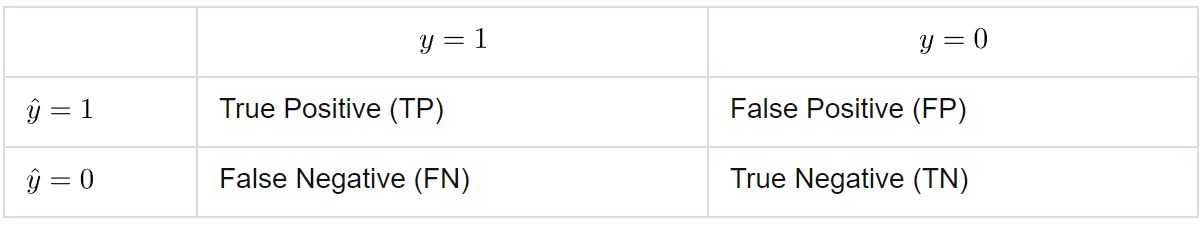
\includegraphics[width=1\textwidth]{pic/matrix.png}
            \caption{Матрица ошибок}
        \end{figure}

        Таким образом, можно определить 4 значения этой матрицы: True Positive
        (TP) или True Negative (TN) "--- количество объектов ''класса A'' или
        количество объектов не из ''класса A'', которые были правильно
        распознаны нейросетью. Величины False Positive (FP) и False Negative
        (FN) "--- количество объектов, которые были неправильно отнесены или не
        отнесены к ''классу А'', соответственно.

        Одними из самых распространенных метрик обучения являются доля
        правильных ответов алгоритма (англ. Accuracy), точность (англ.
        Precision), полнота (англ. Recall) и $F_\beta$.

        Интуитивно понятной, очевидной и почти неиспользуемой метрикой является
        доля правильных ответов алгоритма:

        $$\large accuracy = \frac{TP + TN}{TP + TN + FP + FN}$$

        Эта метрика бесполезна в задачах с неравными классами "--- при
        определении всех элементов выборки как объектов преобладающего класса
        значение метрики будет расти с увеличением разницы в количестве объектов
        между преобладающим и иными классами.

        Для оценки качества работы алгоритма на каждом из классов по отдельности
        вводятся точность и полнота:

        $$\large precision = \frac{TP}{TP + FP}$$

        $$\large recall = \frac{TP}{TP + FN}$$

        Precision можно интерпретировать как долю объектов, названных
        классификатором положительными и при этом действительно являющимися
        положительными, а Recall показывает, какую долю объектов положительного
        класса из всех объектов положительного класса нашел алгоритм.

        $F_\beta$ (или $F$-мера) является средним гармоническим между двумя
        предыдущими метриками:

        $$\large \ F_\beta = (1 + \beta^2) \cdot \frac{precision \cdot
        recall}{(\beta^2 \cdot precision) + recall}$$

        Изменение значение параметра $\beta$ в формуле определяет то, насколько
        для определения метрики важно значение той или иной метрики: Precision
        или Recall.


\section{Практическая часть}

    \subsection{Описание инструментов и библиотек программной реализации}

        В течение последнего десятилетия язык программирования Python показал
        себя как широко используемый язык для создания, обучения и работы с
        моделями машинного и глубокого обучения с помощью таких инструментов,
        как scikit-learn, TensorFlow и PyTorch, которые в основном предоставляют
        интерфейсы Python \cite{fwtf}, \cite{fwtf} и \cite{fwpytorch}.
        Совокупность библиотек NumPy, Pandas, Matplotlib, seaborn и Jupyter
        Notebook упрощает анализ результатов обучения моделей нейросетей и
        исследование данных \cite{python}, \cite{fwnumpy}, \cite{fwpandas},
        \cite{fwjupyter}.

        % pandas
        Вопрос способа сопоставления текста комментария к фильму и целевого
        признака решается с помощью представления этой связи в виде таблицы, в
        которой в первой колонке указывается содержимое комментария, а во второй
        колонке записывается значение целевого признака (то есть, ''позитивный''
        отзыв или ''негативный''). Способ хранения таких данных не важен, и
        основным требованием к нему является простота способа считывания данных,
        поэтому в качестве формата для хранения таблицы был выбран CSV
        (Comma-Separated Values) "--- текстовый формат, предназначенный для
        представления табличных данных, где значения полей одной строки
        разделяются между собой запятыми. Для работы с данными такого вида на
        языке Python самым распространенным является инструментарий библиотеки
        Pandas.

        % nltk
        Чтобы осуществить предобработку текстов комментариев с помощью описанных
        методов (мешок слов, стемминг, лемматизация и т.д.), был использован
        Natural Language Toolkit (или NLTK) "--- набор библиотек и программ,
        написанных на языке программирования Python, для символьной и
        статистической обработки естественного языка англоязычных текстов. 

        % sklearn
        Для применения описанных выше алгоритмов машинного обучения был
        использован инструмент scikit-learn (ранее scikits.learn, также
        известная как sklearn) "--- бесплатная библиотека машинного обучения для
        языка программирования Python. Она представляет собой модуль,
        объединяющий широкий спектр современных алгоритмов машинного обучения
        для задач среднего масштаба с учителем и без учителя. Этот пакет методов
        ориентирован на предоставление машинного обучения неспециалистам с
        использованием языка высокого уровня общего назначения. Акцент делается
        на простоте использования, производительности, доступной документации и
        согласованности API. С помощью данного инструмента были реализованы и
        обучены все алгоритмы (наивный байесовский классификатор, метод опорных
        векторов, логистическая регрессия), а также получены значения всех
        метрик (accuracy, precision, recall, f-score) и матрицы ошибок.

        % plt sns
        Для проверки качества обученных алгоритмов была использована библиотека
        Matplotlib "--- модуль для создания статических, анимированных и
        интерактивных визуализаций на Python. Являясь инструментом построения
        графиков для Python и его расширения для числовой математики NumPy, он
        предоставляет объектно-ориентированный API для встраивания графиков в
        приложения с помощью инструментов общего назначения с графическим
        интерфейсом, таких как Tkinter, wxPython, Qt или GTK. Дополнительные
        настройки отрисовки графиков позволял осуществить Seaborn — ещё одна
        библиотека визуализации данных, основанная на matplotlib. Она
        предоставляет высокоуровневый интерфейс для рисования привлекательных и
        информативных статистических графиков. При выполнении данной
        исследовательской работы с помощью Matplotlib и Seaborn было
        осуществлено построение матриц ошибок с подробной легендой.

    \subsection{Описание набора данных для обучения и теста}

        В качестве используемого набора данных для решения поставленной задачи
        была взята выборка ''IMDB Dataset''. Это набор данных для бинарной
        классификации тональности текста, содержащий значительно больше данных,
        чем предыдущие эталонные наборы данных, представленные от IMDB. IMDb
        "--- это онлайн-база данных, содержащая информацию о фильмах,
        телесериалах, подкастах, домашнем видео, видеоиграх и потоковом
        онлайн-контенте, включая актеров, съемочную группу и личные биографии,
        краткое изложение сюжета, мелочи, рейтинги, а также фанатские и обзоры
        критиков. Набор состоит из 25000 обзоров на популярные фильмы,
        являющимися элементами выборки для обучения, и из 25000 элементов
        выборки для тестирования.

        Набор данных находится в открытом доступе и его можно загрузить как с
        официального сайта IMDB и сайта с ссылкой на научную работу на тему
        вектора слов, так и с других различных форумов и сайтов для машинного и
        глубокого обучения. В частности, для обучения алгоритмов машинного
        обучения, описываемых в данной работе, такая коллекция комментариев с
        соответствующими определенными тональностями, представленная в файле
        формата CSV, была взята с Kaggle "--- платформы для проведения
        соревнований по анализу данных \cite{dataset3}.

        Пример двух элементов выборки из CSV-файла:
        
        \begin{minted}[fontsize=\footnotesize]{text}
            review,sentiment
            "One of the other reviewers...with your darker side.",positive
            "A wonderful little production...terribly well done.",positive
        \end{minted}

    \subsection{Программная реализация}

        Перед применением алгоритмов машинного обучения, была осуществлена
        предобработка данных, которую содержит файл ''preprocessing.py''. Она
        состояла из нескольких этапов.
        
        Сначала осуществлялась очистка содержимого комментариев от
        малоиспользуемых, не соответствующих задаче символов и текстовых
        структур:

        \begin{enumerate}
            \item Удаление ненужных символов из текстов;
            \item Изменение кодировки текста комментария на UNICODE;
            \item Удаление частей ссылок (подпись ''http'' и т.д.);
            \item Удаление символов-эмодзи;
            \item Удаление спецсимволов и квадратных скобок из текста;
            \item Приведение текстов к нижнему регистру.
        \end{enumerate}

        Второй этап предобработки представлял собой удаление стоп-слов из
        элементов выборки. Для этого выбиралось множество стоп-слов, которое
        было сформировано с помощью библиотеки NLTK, и затем по каждому
        комментарию проходился ''фильтр'', который удалял каждое встречающееся
        стоп-слово.

        Третьим и четвертым этапом препроцессинга являлись стемминг и
        лемматизация соответственно.

        Осуществив перечисленные выше действия, получилось сформировать облако
        слов, которое позволило отразить частоту встречающихся в комментариях
        слов.

        \begin{figure}[H]
            \centering
            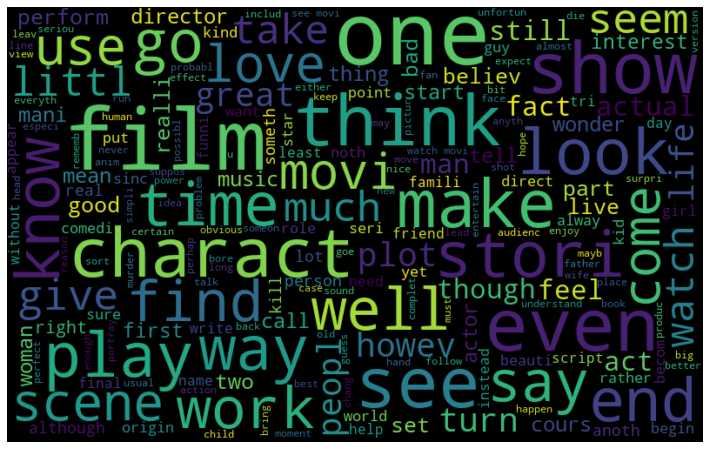
\includegraphics[width=0.8\textwidth]{pic/cloud.png}
            \caption{Облако слов в комментариях после предобработки}
        \end{figure}

        Далее предобработанная выборка сохранялась в отдельный файл формата CSV,
        который использовался в дальнейшем.

        Файл с предобработанной выборкой открывался с помощью программы
        ''algos.py'', в котором загруженный набор данных использовался для двух
        различных экспериментов:
        
        Первый эксперимент начинался с кодировки целевого признака "---
        производилась замена значений ''positive'' и ''negative'' на $1$ и $0$
        соответственно.

        После кодирования самого целевого признака осуществлялось кодирование
        комментариев с помощью функции ''CountVectorizer'' "--- улучшенной
        версии ''мешка слов'' из библиотеки sklearn, в которой каждый
        комментарий представлялся вектором, который определял не только факт
        наличия того или иного слова в комментарии, но и его количества (т.е.
        вместо значений $0$ и $1$ для каждого слова из словаря там также
        содержались натуральные числа).

        Затем набор данных разделялся на две части "--- тренировочную и тестовую
        выборки, где 80\% данных случайным образом распределялись в первую
        группу. На первом множестве алгоритмы обучались, а на втором "---
        проверялось качество обучения с помощью определенных метрик.

        Далее поочередно осуществлялось определение, обучение на тренировочном
        наборе, предсказание значений на тестовом наборе и подсчет значений
        матрицы ошибок и всех остальных метрик для алгоритмов:

        \begin{enumerate}
            \item наивный байесовский классификатор;
            \item логистическая регрессия;
            \item метод опорных векторов.
        \end{enumerate}

        Второй эксперимент также включал в себя преобразование элементов
        предобработанной выборки с помощью кодировщика целевого признака, однако
        к комментариям применялся алгоритм преобразования текстов в матрицу
        признаков для $tf \text{-} idf$.

        Векторизованный закодированный набор данных также разделялся на
        тренировочную и тестовую выборки в соотношении 4 к 1, после чего
        осуществлялось обучение и проверка метрик алгоритмов в неотличном от
        первого эксперимента порядке.

    \subsection{Результаты обучения}

        В качестве результатов обучения описанных в работе алгоритмов
        представлена таблица со значениями метрик для каждого из методов
        предобработки текста и каждого классификатора (BoW "--- мешок слов,
        TF-iDF "--- частота слова и обратная частота документа):

        \begin{table}[h]
            \centering
            \begin{tabular}{|l|l|l|l|l|}
            \hline
                                                          & Accuracy & Precision & Recall & F1-score \\ \hline
            BoW, MultinomialNB & 0.8598   & 0.8605    & 0.8598 & 0.8598   \\ \hline
            TF-iDF, MultinomialNB     & 0.8617   & 0.8624    & 0.8617 & 0.8616   \\ \hline
            BoW, Лог. регрессия           & 0.8791   & 0.8791    & 0.8791 & 0.8791  \\ \hline
            TF-iDF, Лог. регрессия               & 0.8948   & 0.8949    & 0.8948 & 0.8947   \\ \hline
            BoW, SVM            & 0.8597   & 0.8597    & 0.8597 & 0.8597      \\ \hline
            TF-iDF, SVM                & 0.8909   & 0.8909    & 0.8909 & 0.8909   \\ \hline
            \end{tabular}
            \captionsetup{justification=centering}
            \caption{Значения метрик}
        \end{table}

        Также были вычислены значения матриц ошибок:

        \begin{figure}[H]
            \centering
            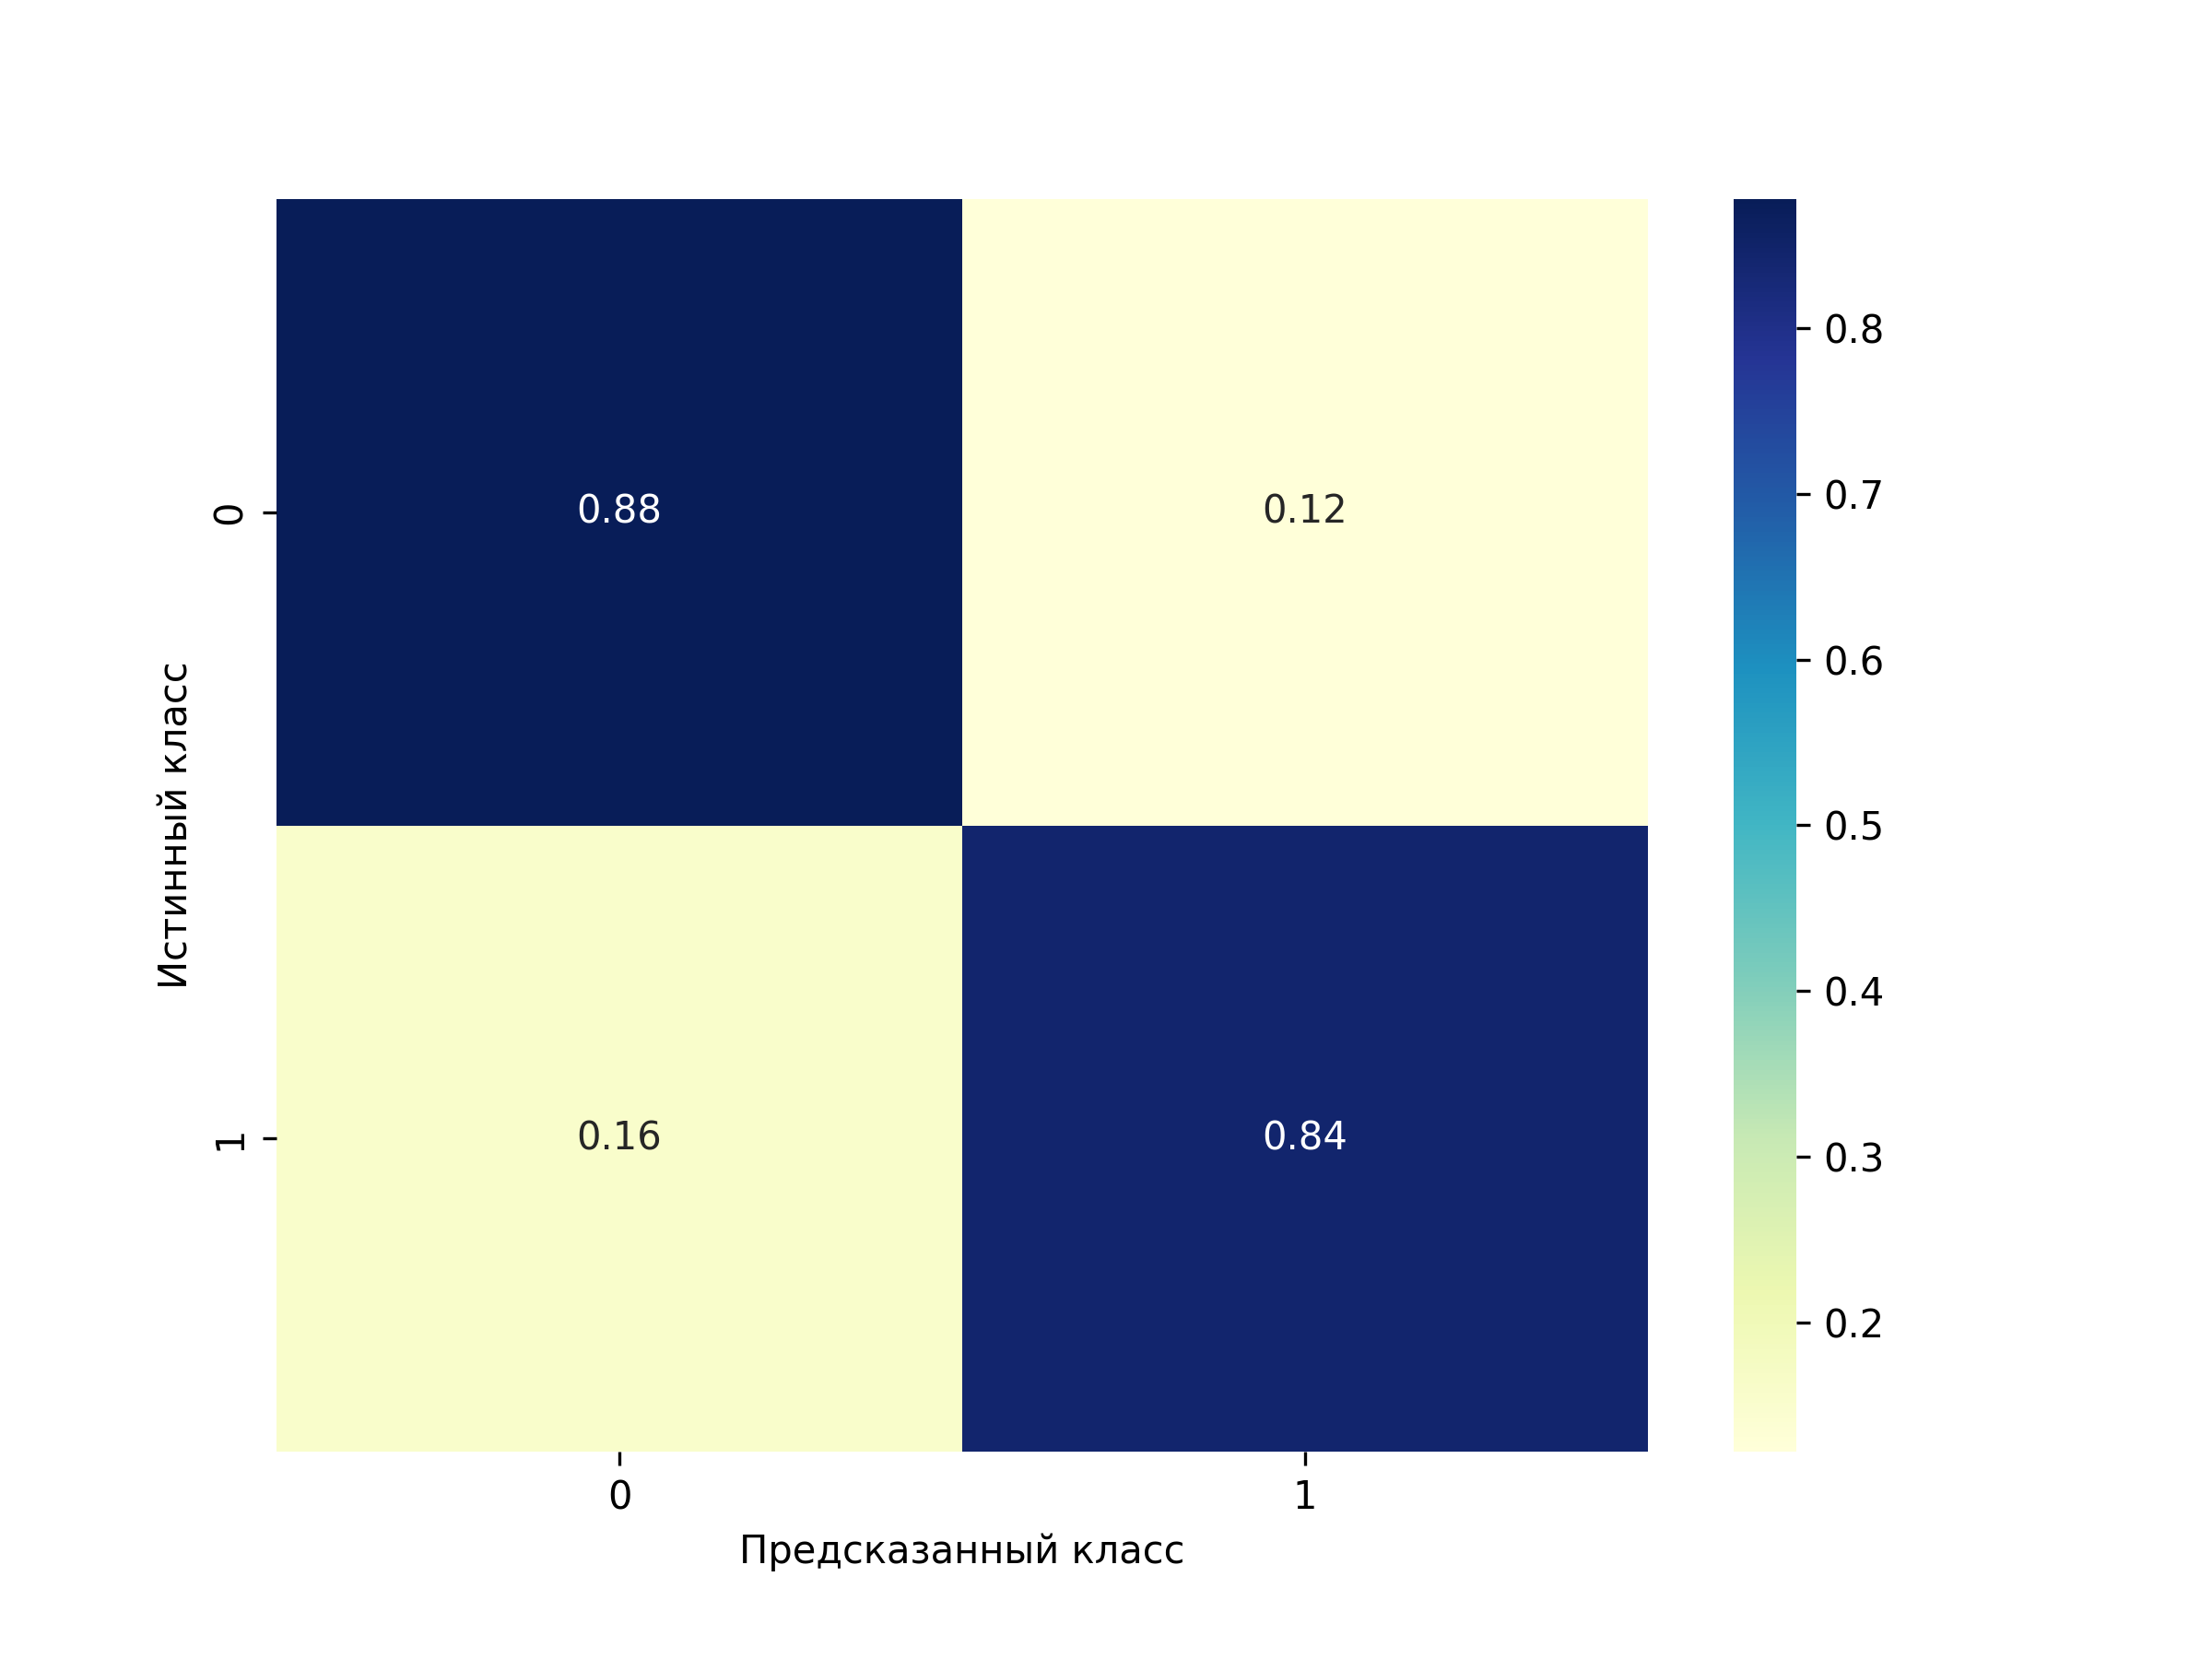
\includegraphics[width=0.8\textwidth]{pic/BOW-NB.png}
            \caption{Матрица ошибок наивного байесовского классификатора после применения мешка слов}
        \end{figure}

        \begin{figure}[H]
            \centering
            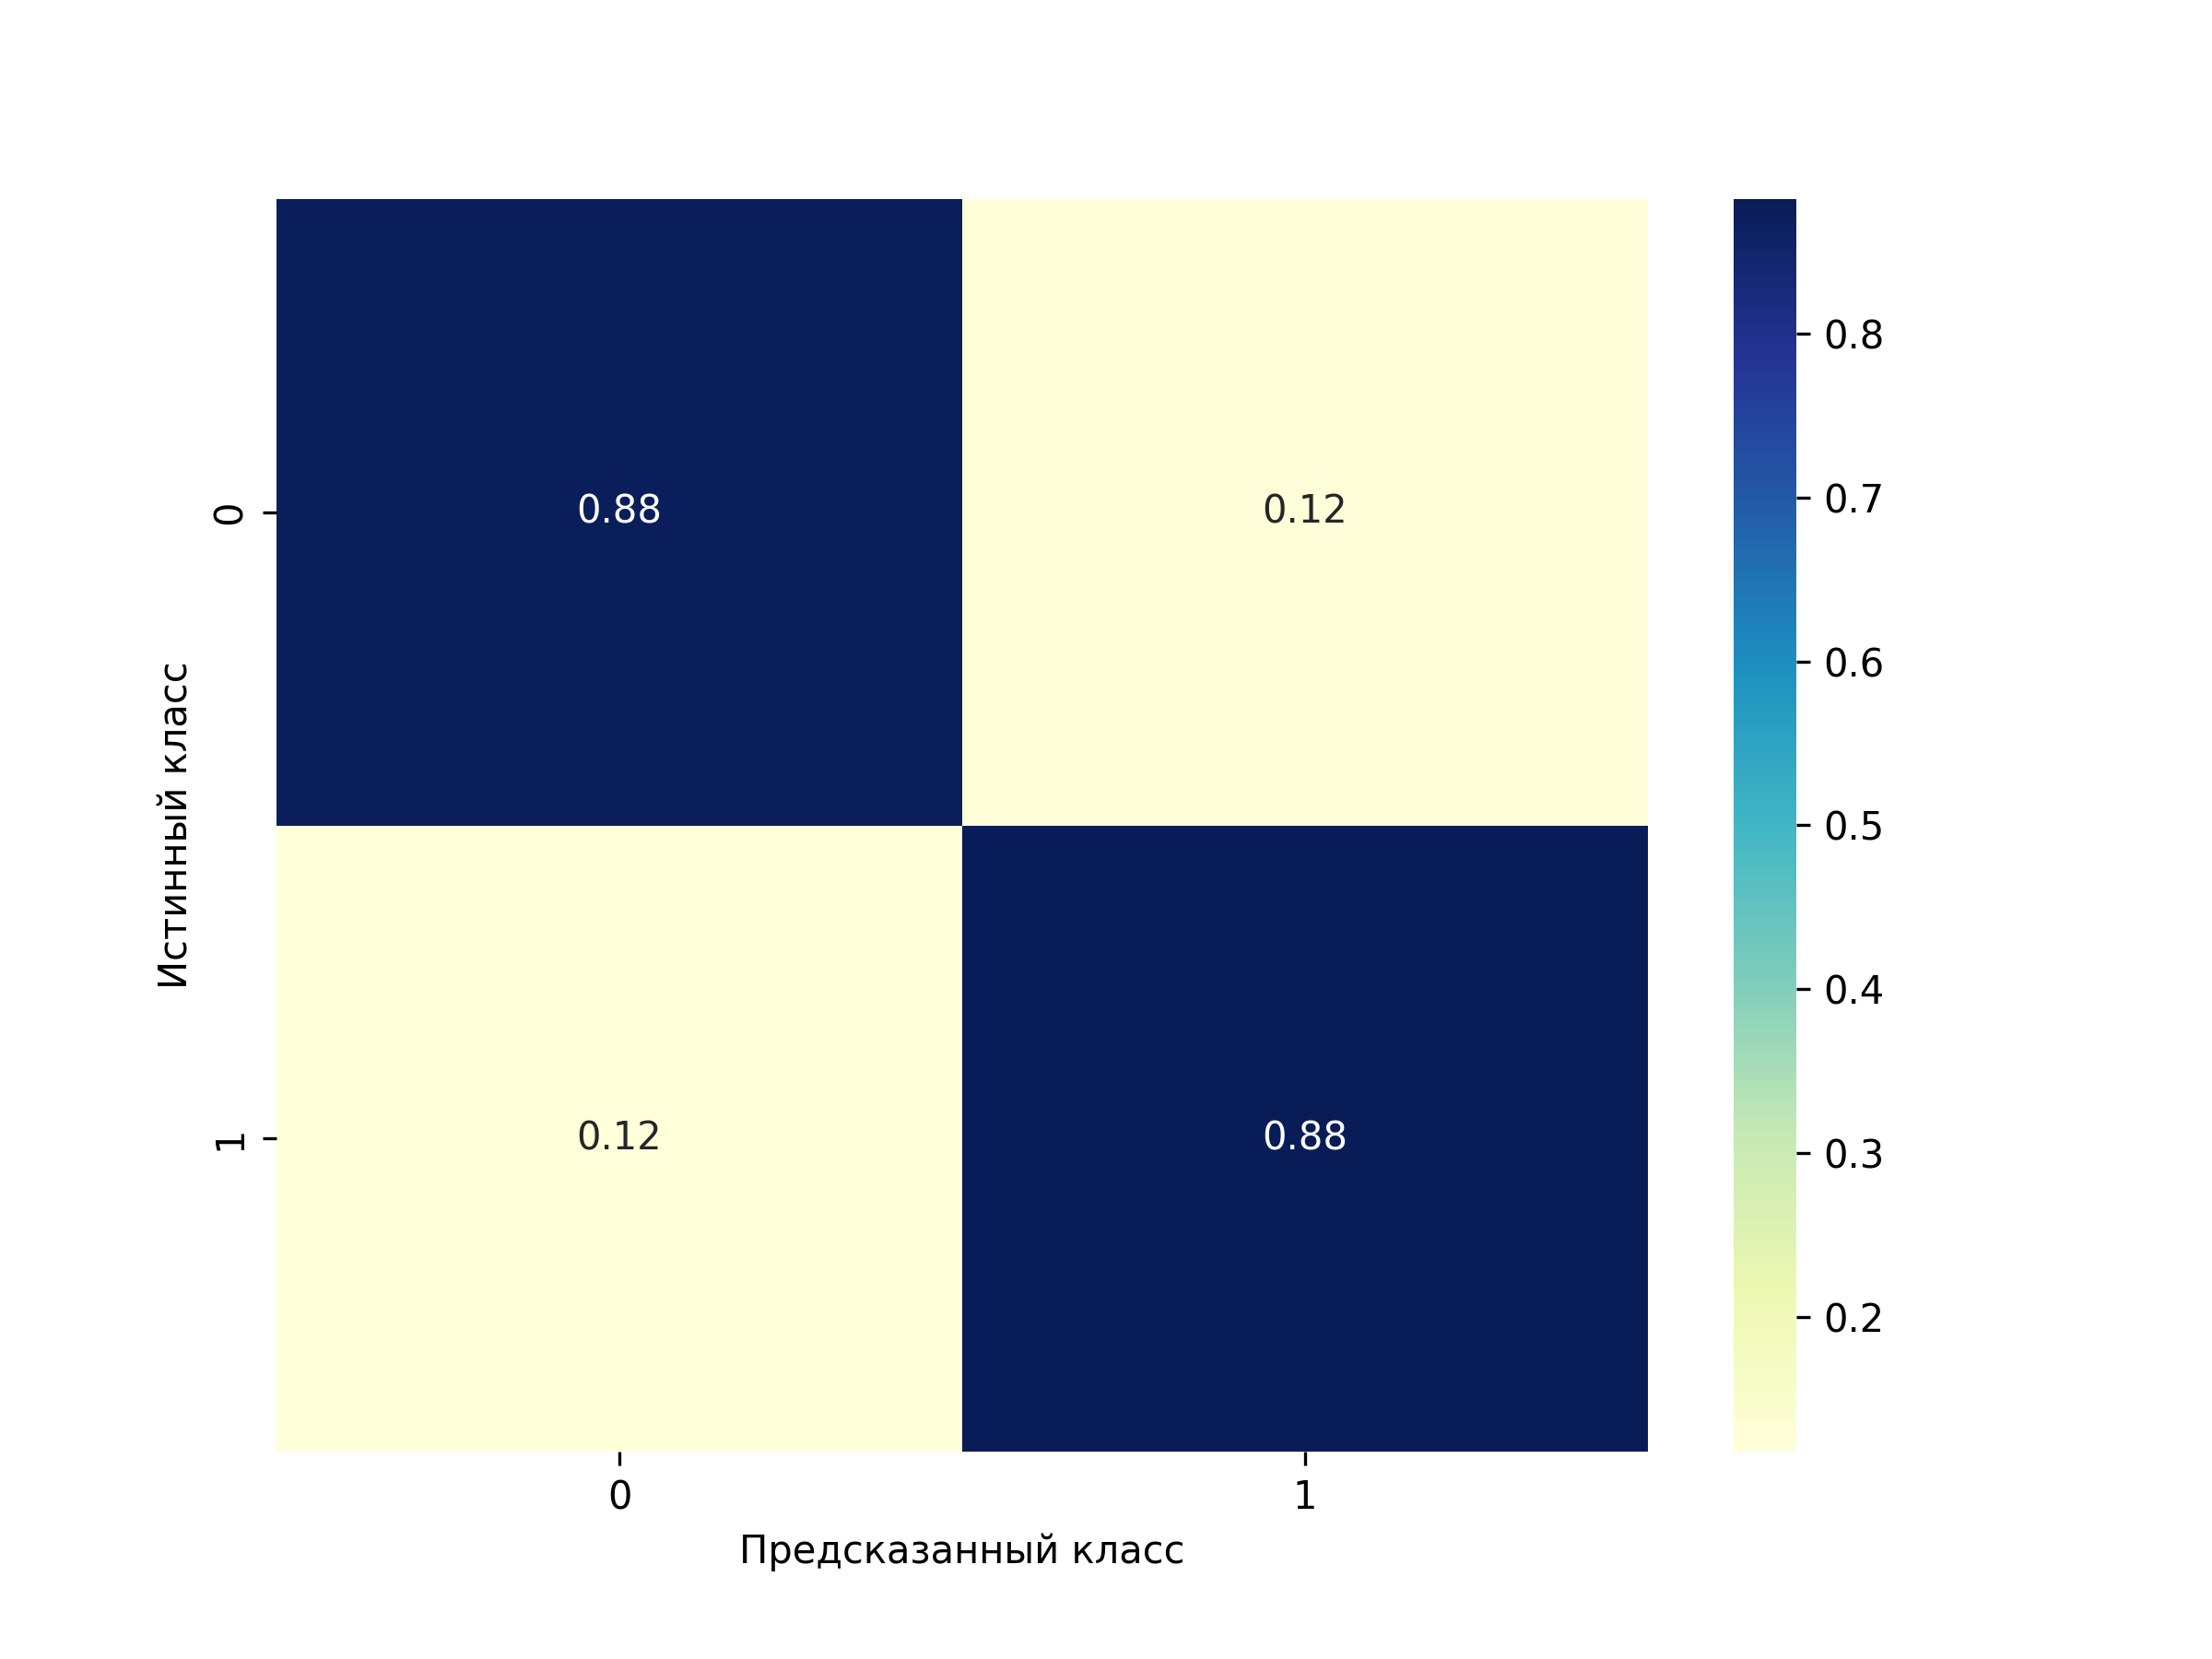
\includegraphics[width=0.8\textwidth]{pic/BOW-LR.png}
            \caption{Матрица ошибок логистической регрессии после применения мешка слов}
        \end{figure}

        \begin{figure}[H]
            \centering
            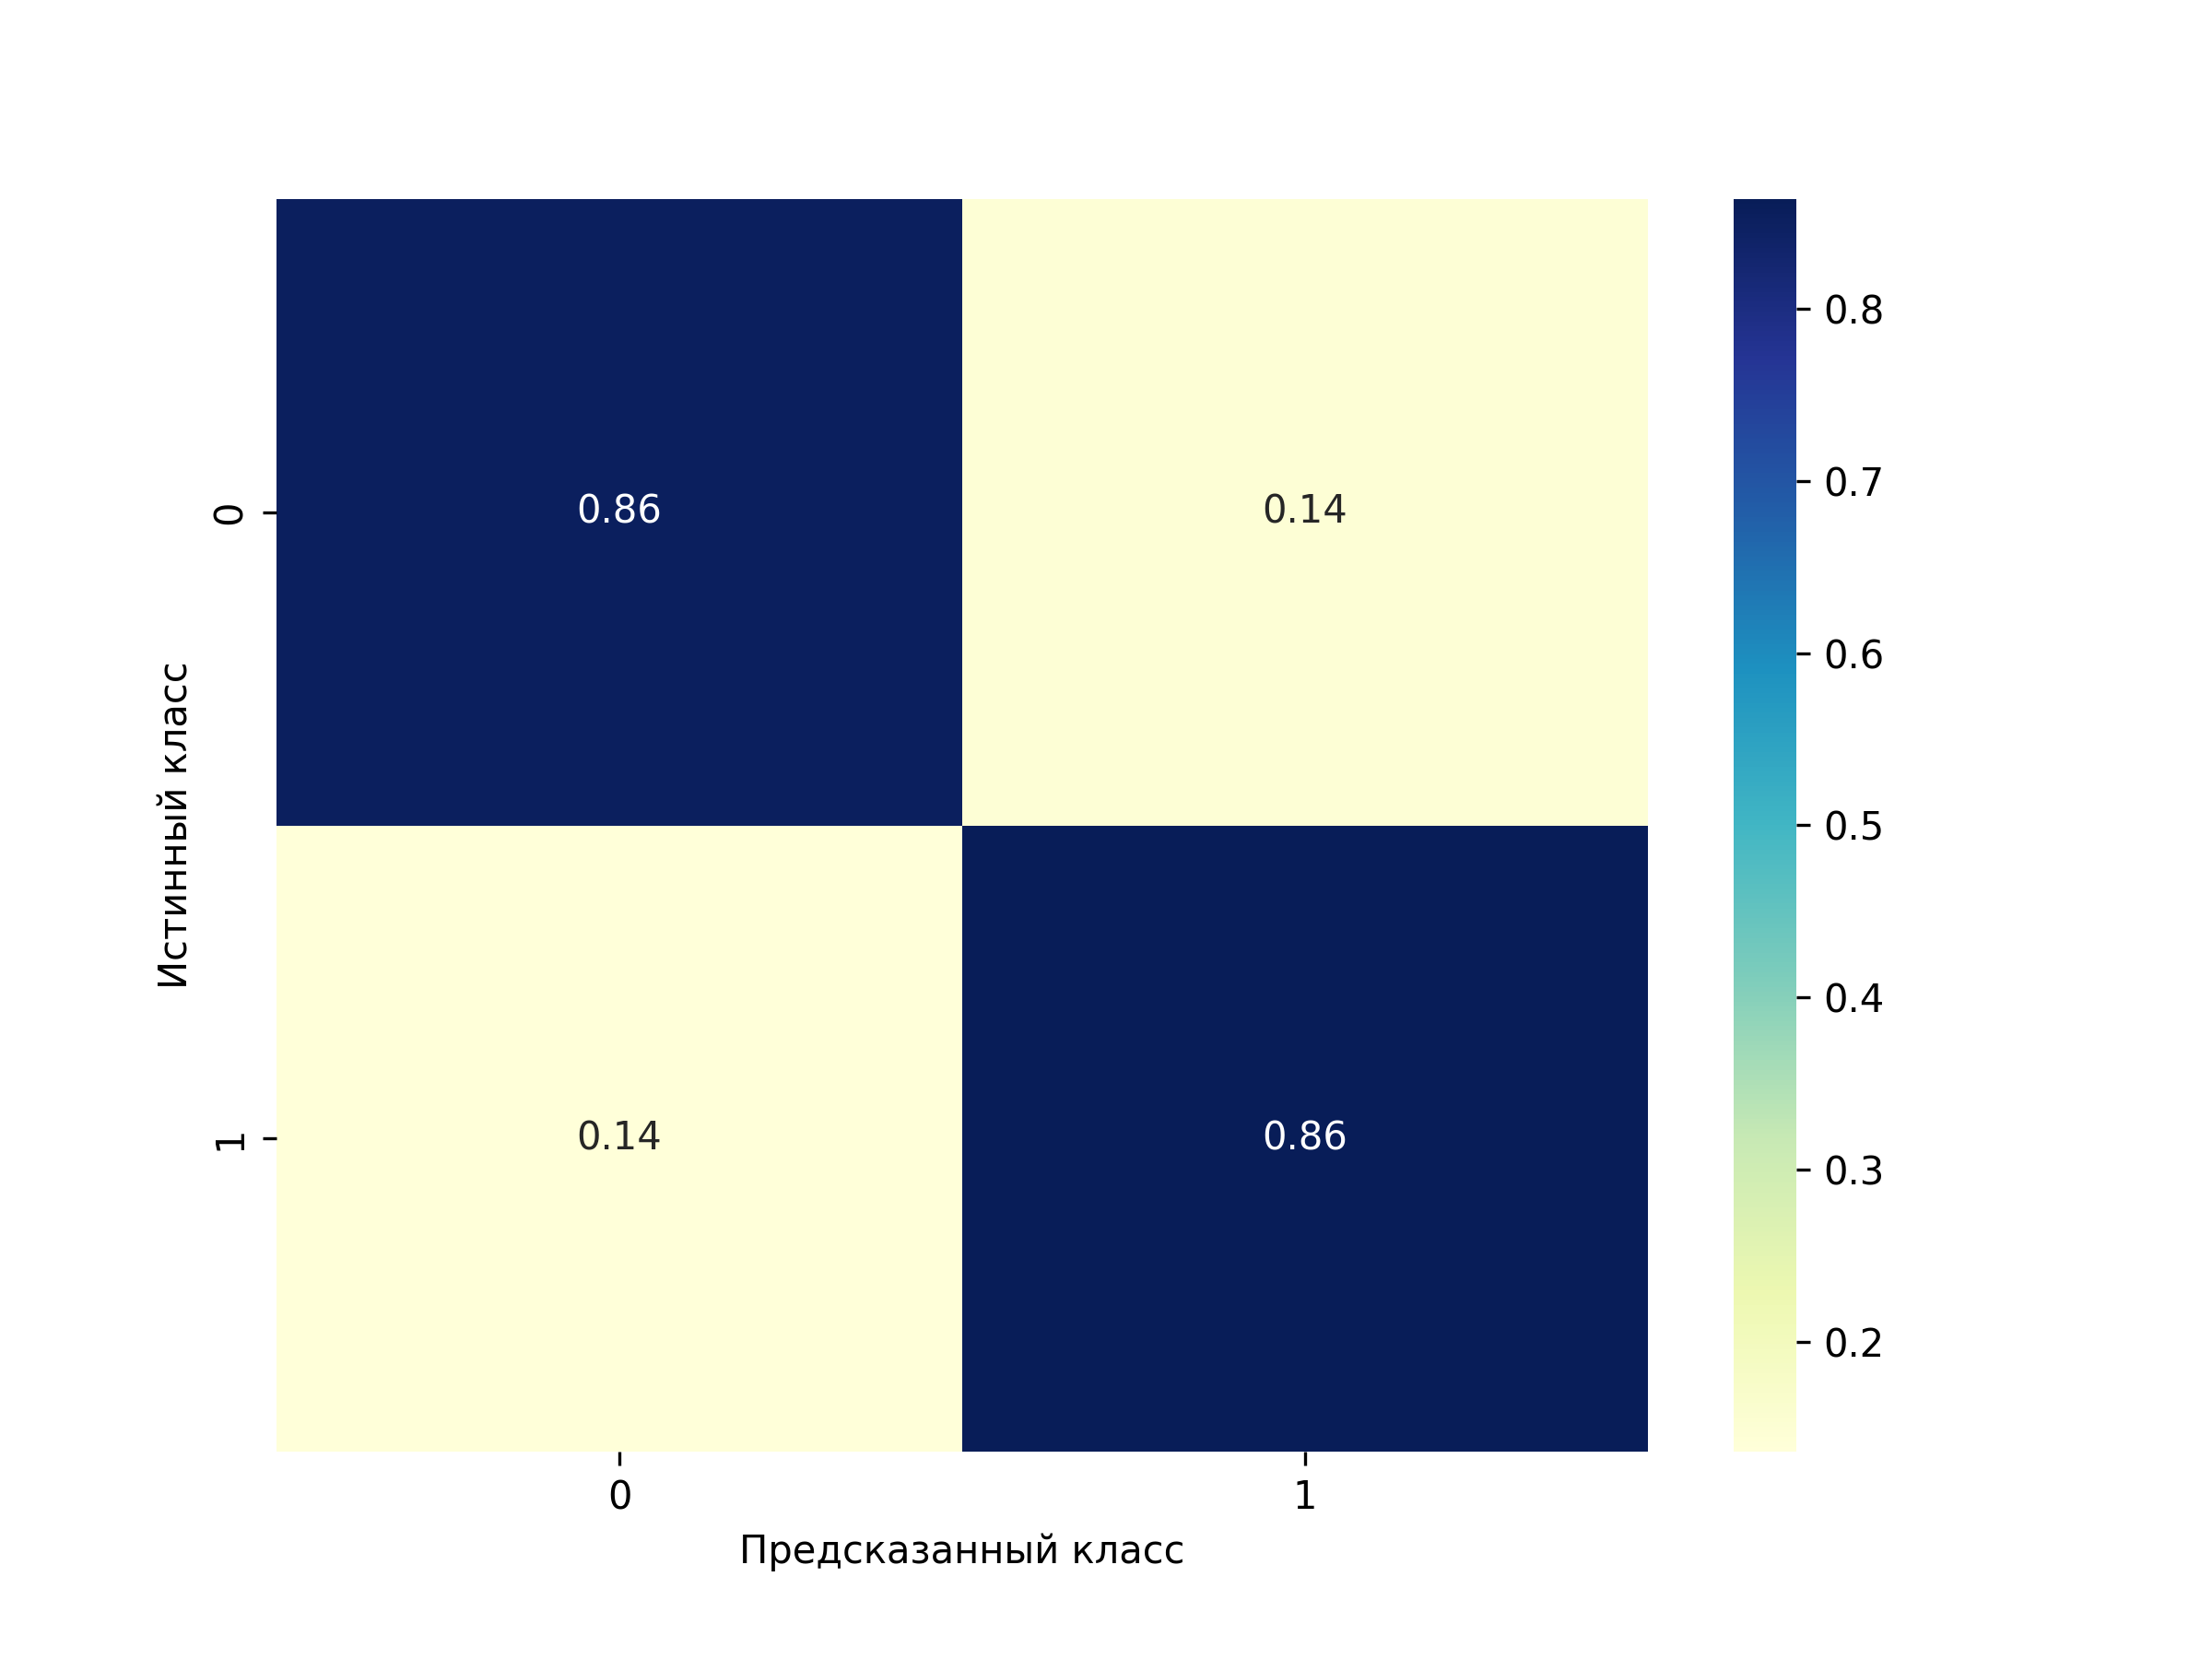
\includegraphics[width=0.8\textwidth]{pic/BOW-SVM.png}
            \caption{Матрица ошибок метода опорных векторов после применения мешка слов}
        \end{figure}

        \begin{figure}[H]
            \centering
            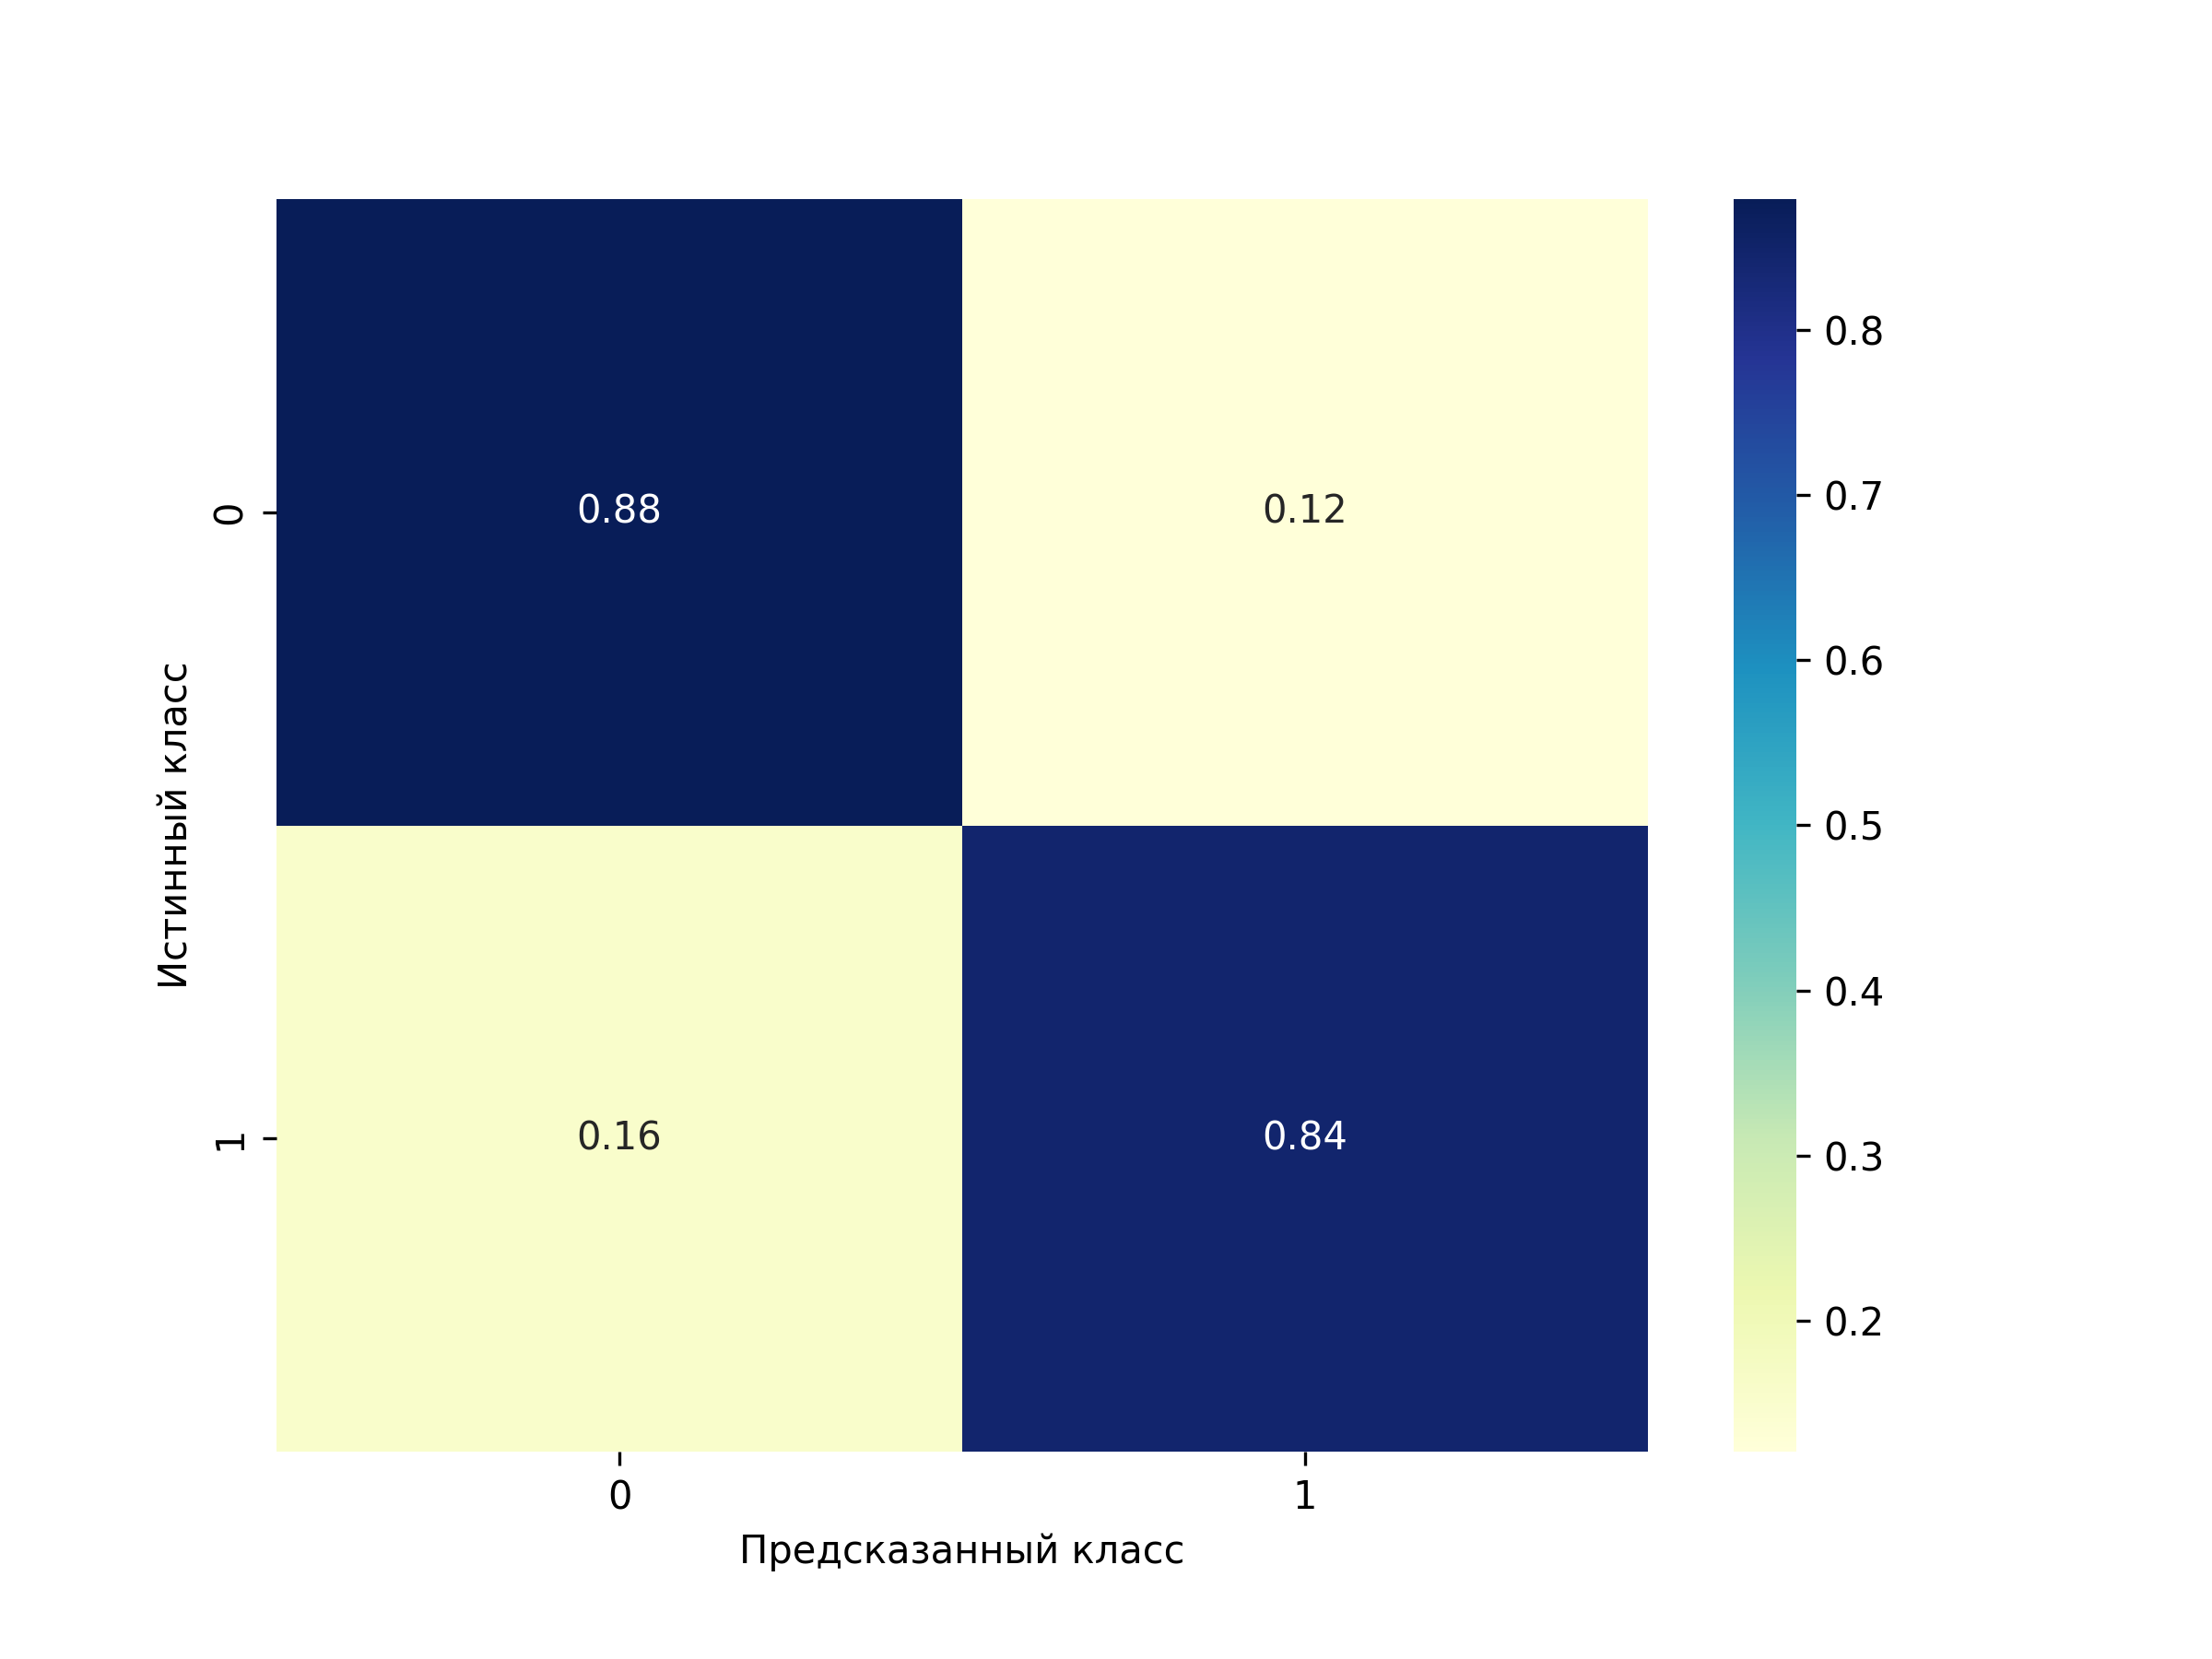
\includegraphics[width=0.8\textwidth]{pic/TFIDF-NB.png}
            \caption{Матрица ошибок наивного байесовского классификатора после создания признаков TF-iDF}
        \end{figure}

        \begin{figure}[H]
            \centering
            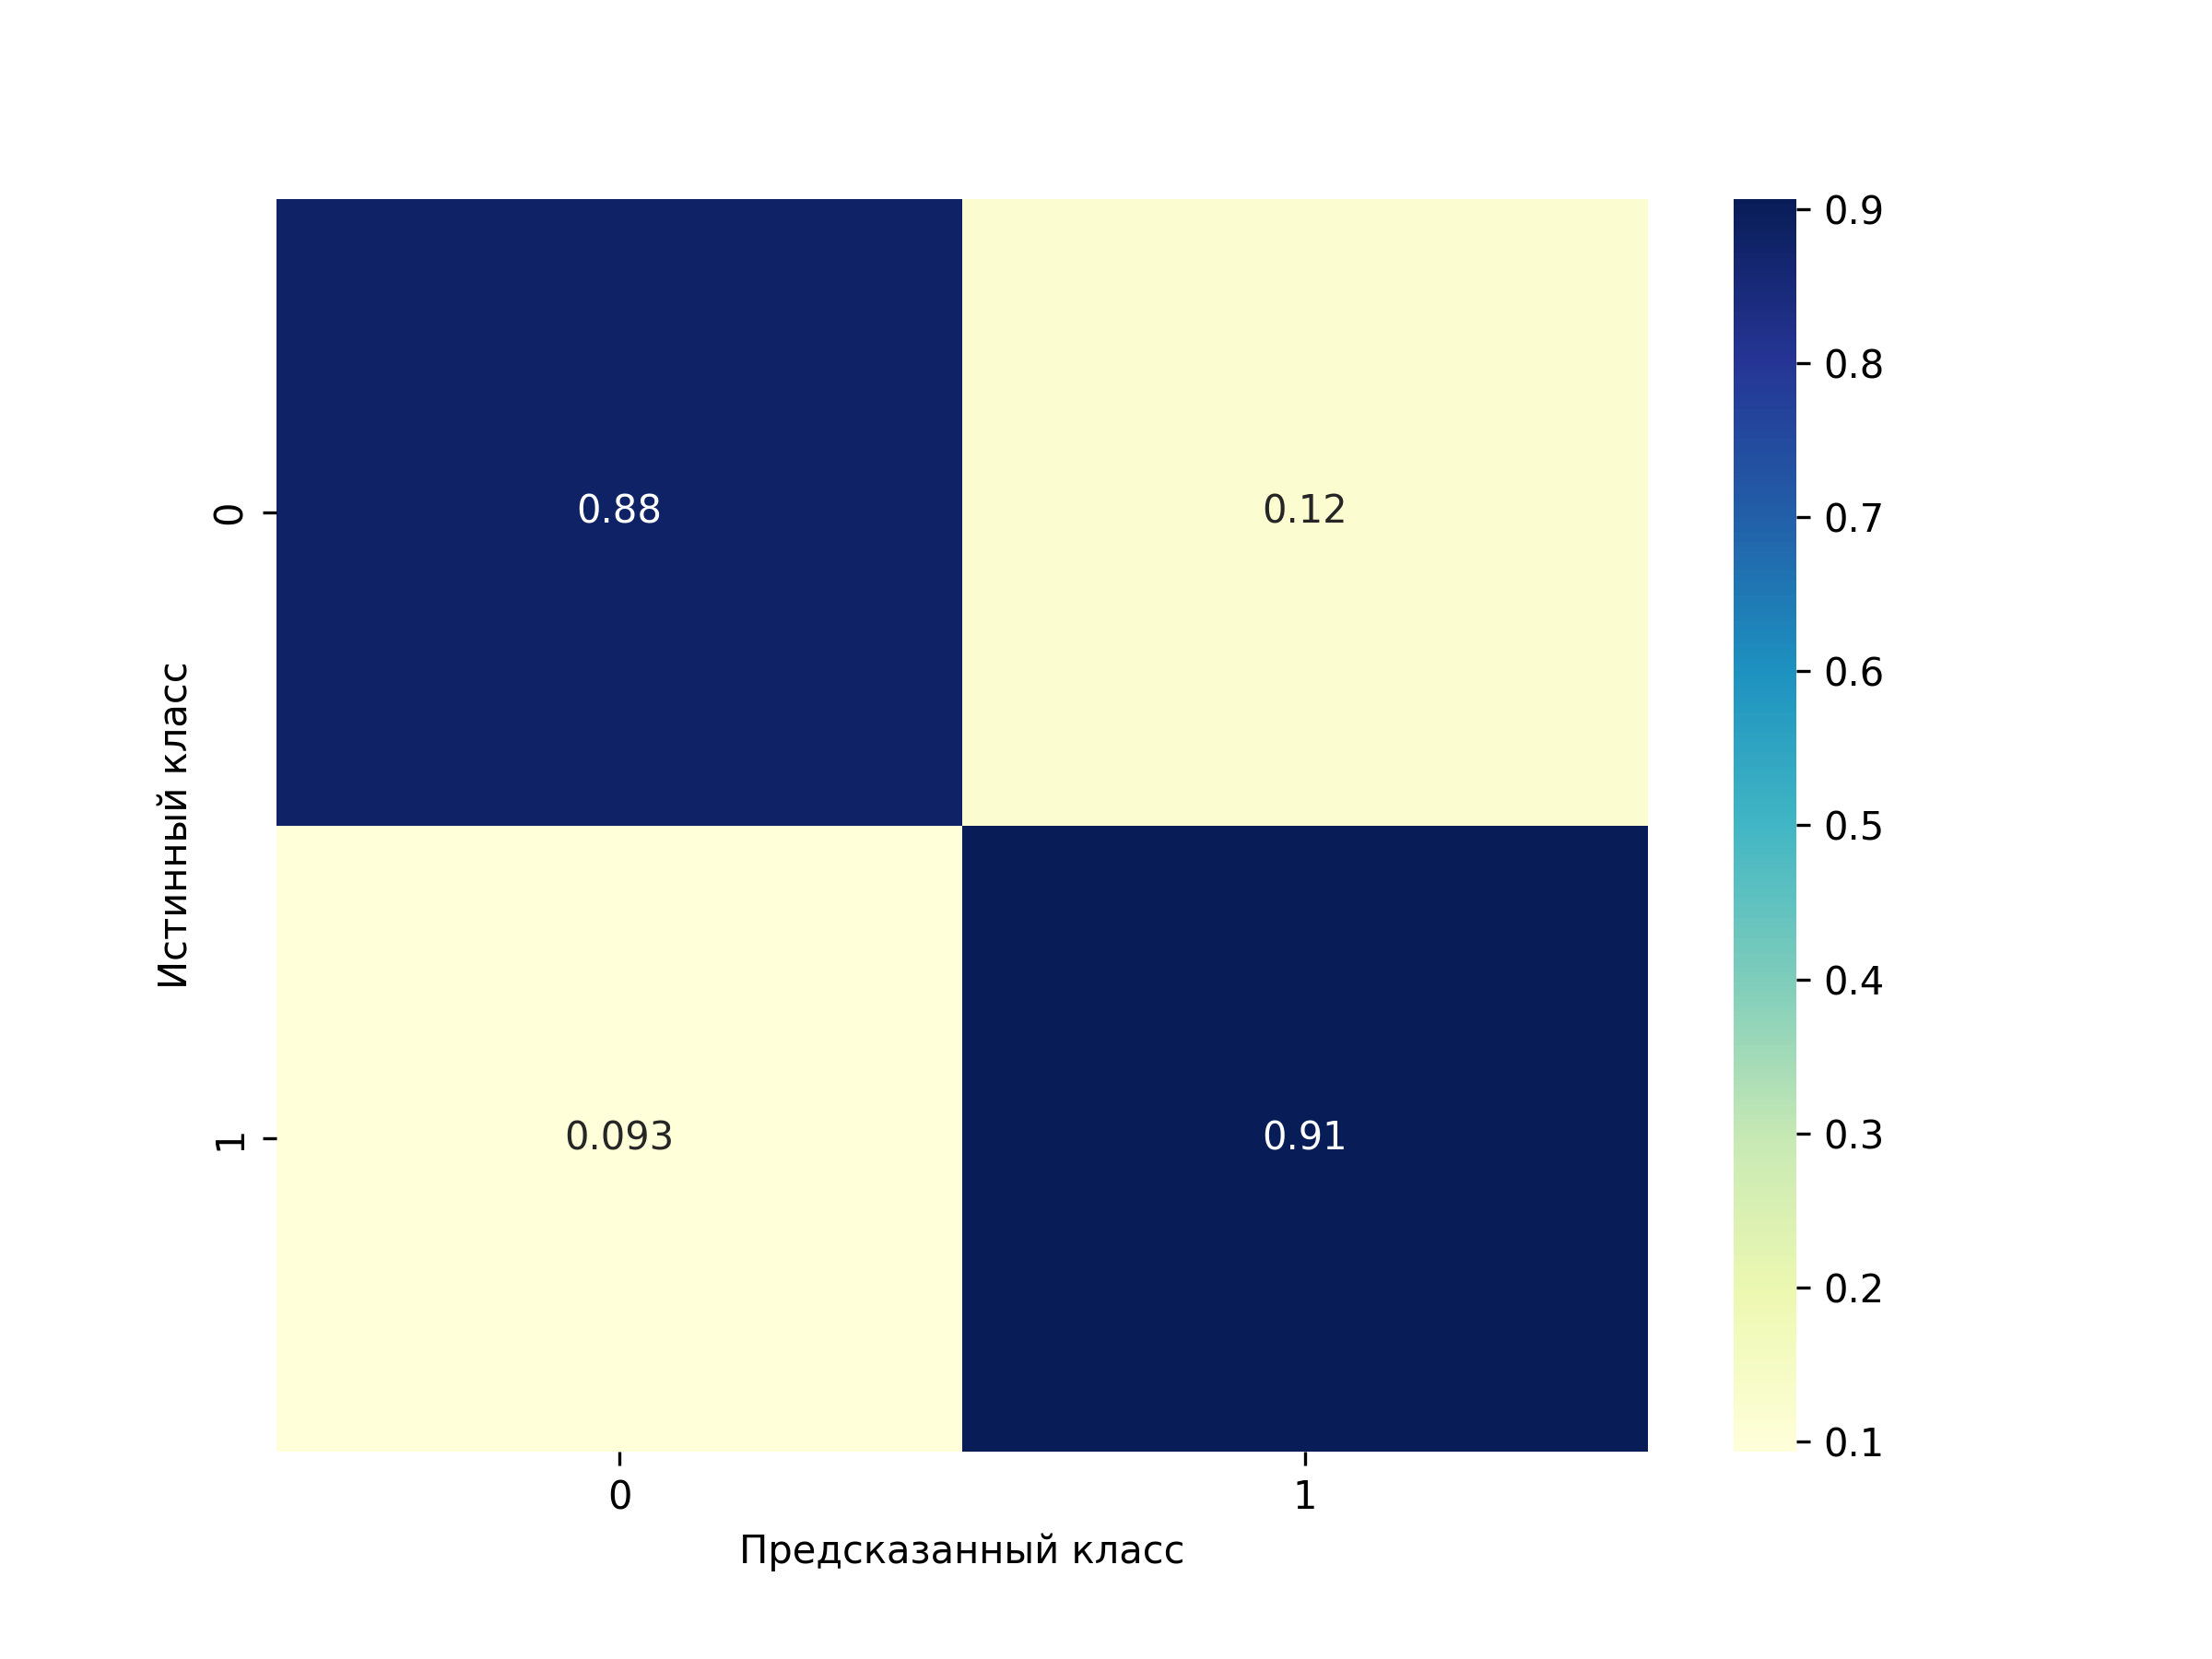
\includegraphics[width=0.8\textwidth]{pic/TFIDF-LR.png}
            \caption{Матрица ошибок логистической регрессии после создания признаков TF-iDF}
        \end{figure}

        \begin{figure}[H]
            \centering
            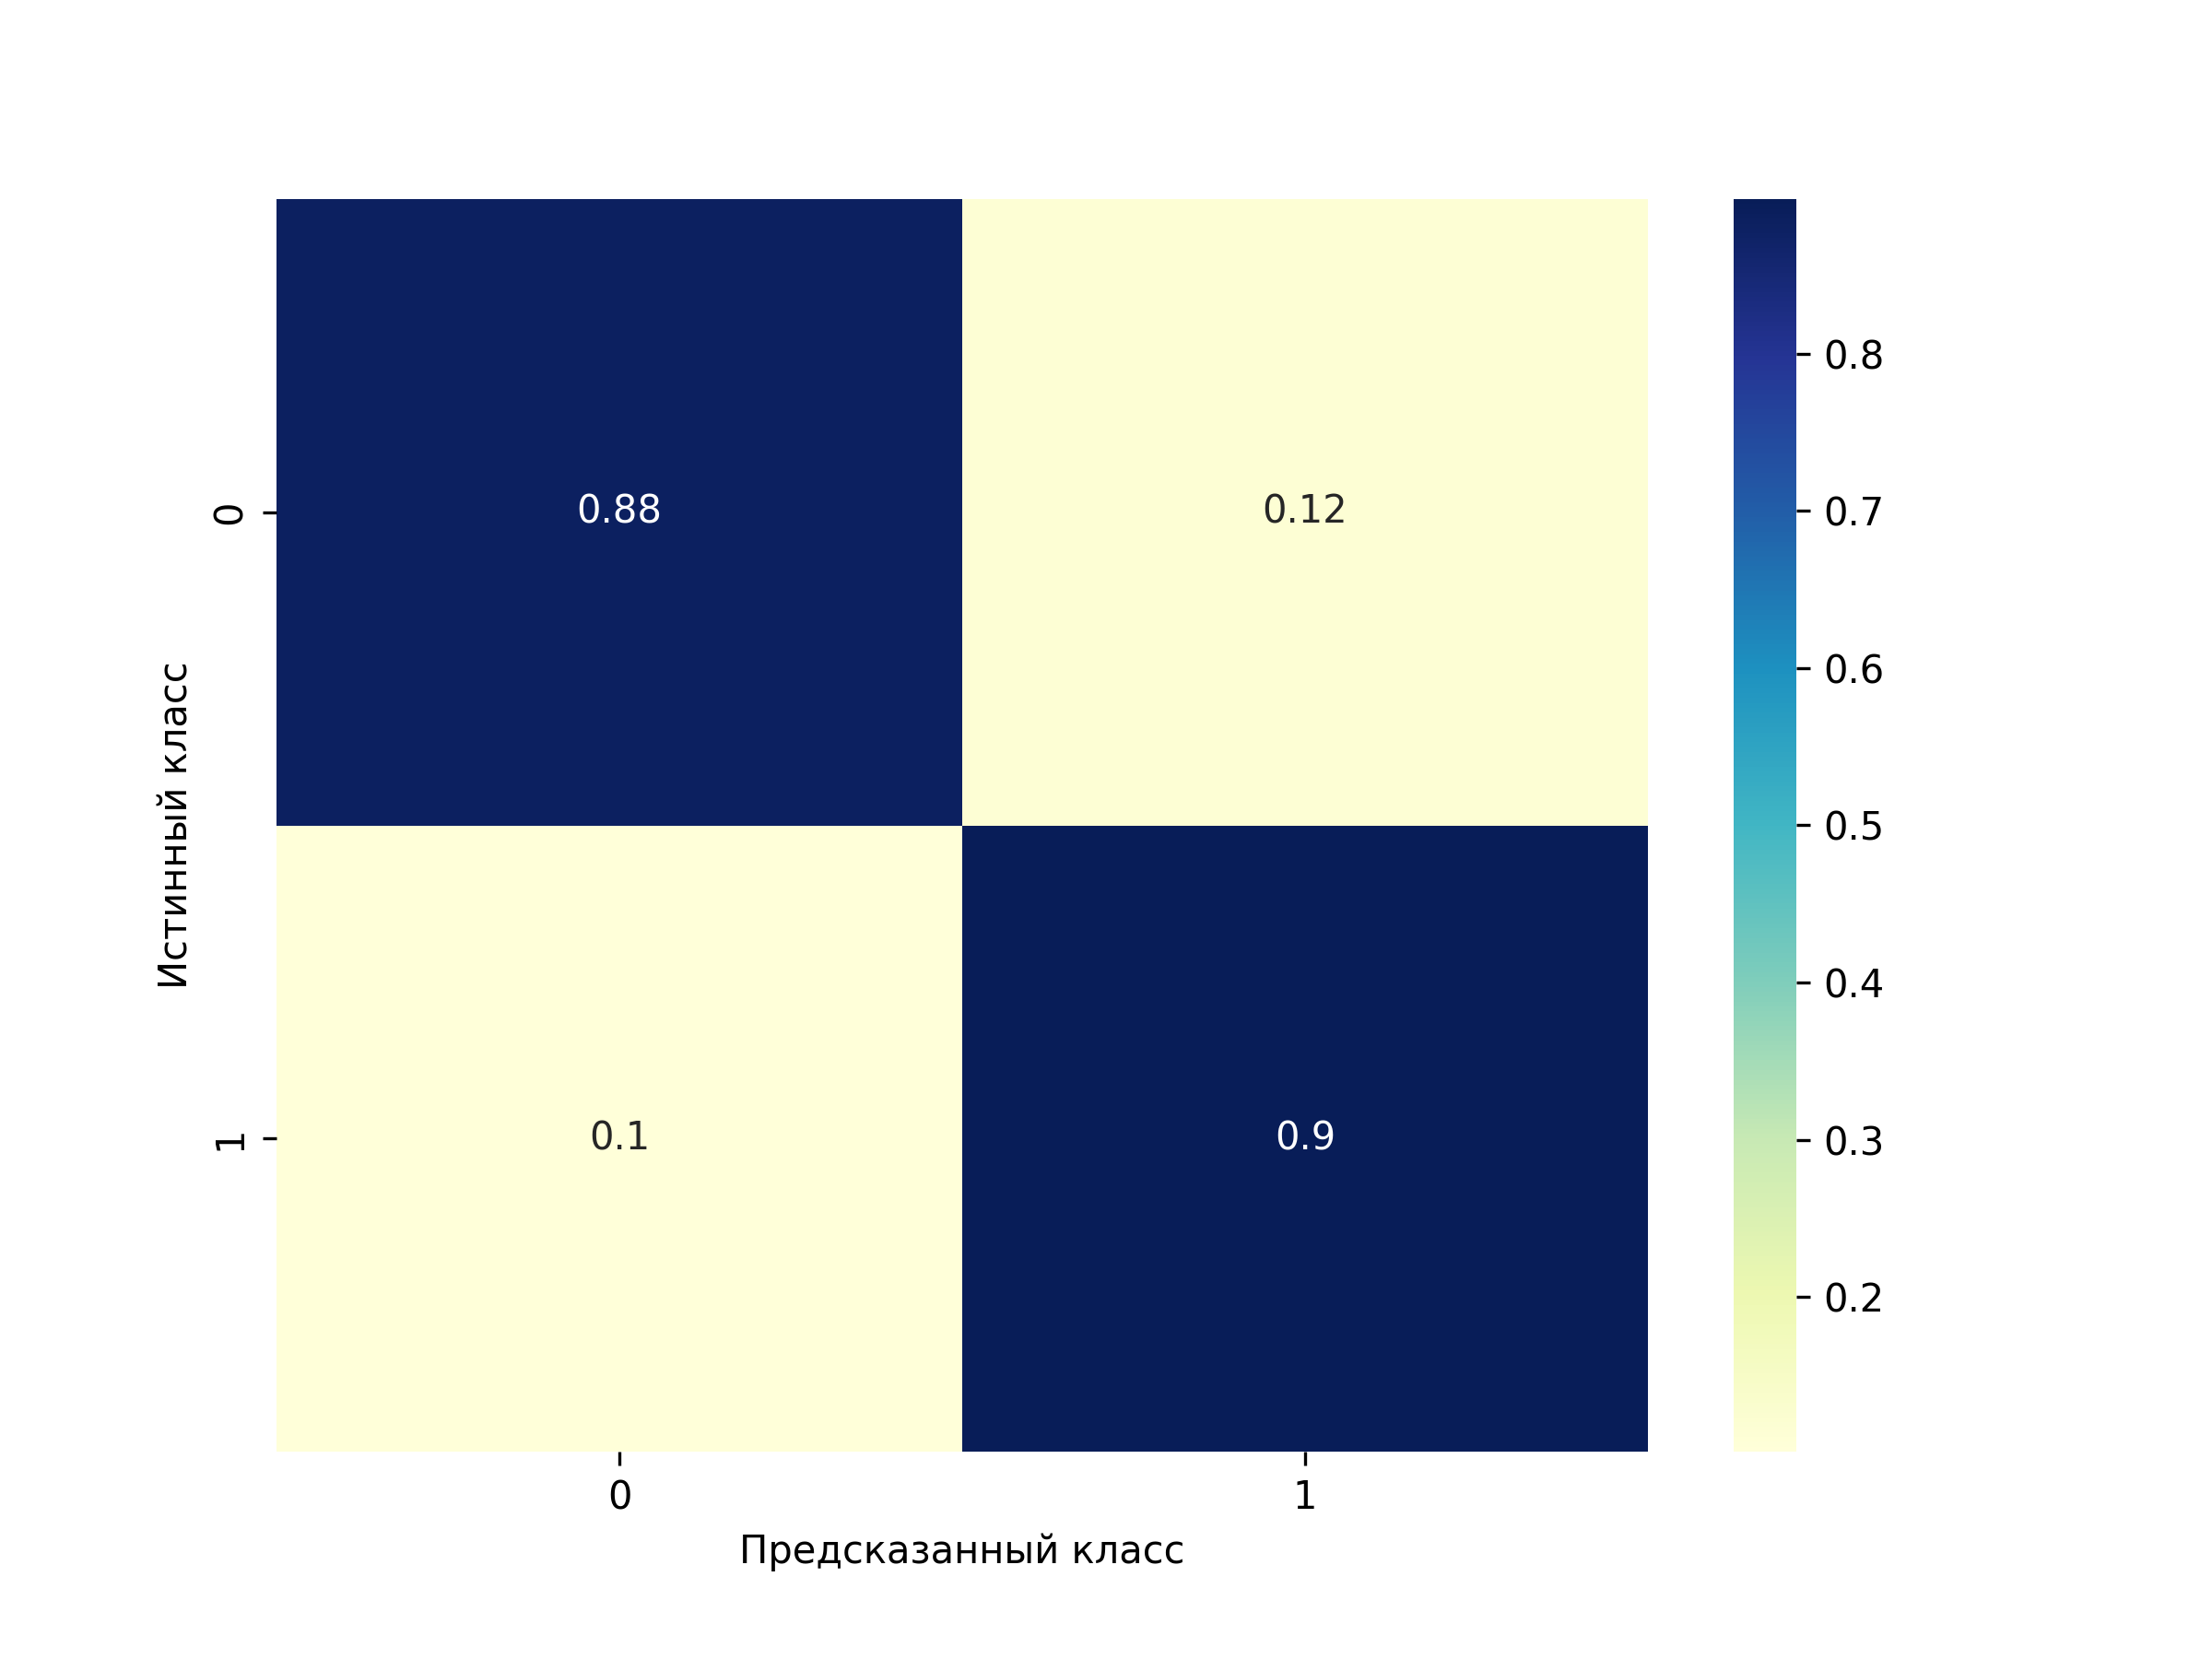
\includegraphics[width=0.8\textwidth]{pic/TFIDF-SVM.png}
            \caption{Матрица ошибок метода опорных векторов после создания признаков TF-iDF}
        \end{figure}

\conclusion

\begin{thebibliography}{99}
    \bibitem{neur} Короткий С., ''Нейронные сети: Основные положения'',
    [Электронный ресурс] : [статья] / URL:
    http://www.shestopaloff.ca/kyriako/Russian/Artificial_Intelligence/Some_publications/Korotky_Neuron_network_Lectures.pdf
    (дата обращения 27.04.2022) Загл. с экрана. Яз. рус.
    
    \bibitem{Gud} Гудфеллоу Я., Бенджио И., Курвилль А., ''Глубокое обучение'',
    г. Москва, Издательство ДМК, 2018 г., Яз. рус.
    
    \bibitem{dataset3} LAKSHMIPATHI N, ''IMDB Dataset of 50K Movie Reviews'',
    [Электронный ресурс] : [статья] / URL
    https://www.kaggle.com/datasets/lakshmi25npathi/imdb-dataset-of-50k-movie-reviews
    (дата обращения 29.04.2023) Загл. с экрана. Яз. англ.

    % Bag of words

    % tf-idf
    % https://arxiv.org/abs/2001.09896

    % naive bayes
    % https://scikit-learn.org/stable/modules/naive_bayes.html

    % Logistic regression
    % Hosmer, David W.; Lemeshow, Stanley (2000). Applied Logistic Regression

    % 

    \bibitem{fwpandas} ''pandas'' [Электронный ресурс] : [сайт] / URL:
    https://pandas.pydata.org/ (дата обращения 17.05.2022) Загл. с экрана. Яз.
    англ.

\end{thebibliography}

\appendix

    \section{Код \texttt{preprocessing.py}}
    \inputminted{py}{../movie-review-data/preprocessing.py}

    \section{Код \texttt{algos.py}}
    \inputminted{py}{../movie-review-data/algos.py}

\end{document}
